\documentclass[aspectratio=169]{beamer}
\usepackage[portuges]{babel}
\usepackage[utf8]{inputenc}
\usepackage[alf]{abntex2cite}	
\usepackage[portuguese, linesnumbered, vlined, titlenumbered, ruled]{algorithm2e}
\usepackage{beamerthemesplit}
\usepackage{multirow}
\usepackage{scalefnt}
\SetKwRepeat{Registro}{registro \{}{\}}%
\newcommand{\Int}{\KwSty{int}}

\usepackage{tikz}
\usetikzlibrary{matrix,backgrounds,matrix,positioning,arrows}
\usetikzlibrary{patterns,arrows,decorations.pathreplacing}
% The Beamer class comes with a number of default slide themes
% which change the colors and layouts of slides. Below this is a list
% of all the themes, uncomment each in turn to see what they look like.

%\usetheme{default}
%\usetheme{AnnArbor}
%\usetheme{Antibes}
%\usetheme{Bergen}
%\usetheme{Berkeley}
%\usetheme{Berlin}
%\usetheme{Boadilla}
%\usetheme{CambridgeUS}
%\usetheme{Copenhagen}
%\usetheme{Darmstadt}
%\usetheme{Dresden}
%\usetheme{Frankfurt}
%\usetheme{Goettingen}
%\usetheme{Hannover}
%\usetheme{Ilmenau}
%\usetheme{JuanLesPins}
%\usetheme{Luebeck}
\usetheme{Madrid}
%\usetheme{Malmoe}
%\usetheme{Marburg}
%\usetheme{Montpellier}
%\usetheme{PaloAlto}
%\usetheme{Pittsburgh}
%\usetheme{Rochester}
%\usetheme{Singapore}
%\usetheme{Szeged}
%\usetheme{Warsaw}

% As well as themes, the Beamer class has a number of color themes
% for any slide theme. Uncomment each of these in turn to see how it
% changes the colors of your current slide theme.

%\usecolortheme{albatross}
%\usecolortheme{beaver}
%\usecolortheme{beetle}
%\usecolortheme{crane}
\usecolortheme{dolphin}
%\usecolortheme{dove}
%\usecolortheme{fly}
%\usecolortheme{lily}
%\usecolortheme{orchid}
%\usecolortheme{rose}
%\usecolortheme{seagull}
%\usecolortheme{seahorse}
%\usecolortheme{whale}
%\usecolortheme{wolverine}

%\setbeamertemplate{footline} % To remove the footer line in all slides uncomment this line
%\setbeamertemplate{footline}[page number] % To replace the footer line in all slides with a simple slide count uncomment this line

%\setbeamertemplate{navigation symbols}{} % To remove the navigation symbols from the bottom of all slides uncomment this line


\usepackage{graphicx} % Allows including images
\usepackage{booktabs} % Allows the use of \toprule, \midrule and \bottomrule in tables

%----------------------------------------------------------------------------------------
%	TITLE PAGE
%----------------------------------------------------------------------------------------
%%%%%%%%%%%%%%%%%%%%%%%%%%%%%%%%%%%%%%%%%%%%%%%%%%%%%%%%%%%%%%%%%%%%%%%%%%%%%%%%%%%%%%%%%

\title[Algoritmos de Ordenação]{Algoritmos e Estrutura de Dados II}
\subtitle{Algoritmos de Ordenação}
\author[Frederico Santos de Oliveira]{prof. Frederico Santos de Oliveira}
\institute[UFMT]{Universidade Federal de Mato Grosso\\ Instituto de Engenharia}
\date{}

\begin{document}

%------------------------------------------------
\begin{frame}
\titlepage % Print the title page as the first slide

\begin{figure}[!h]
  \centering
  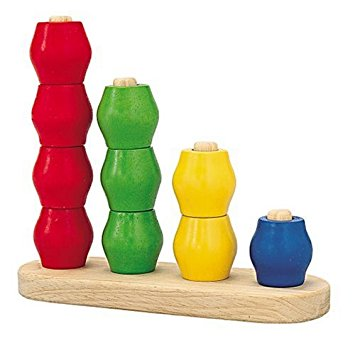
\includegraphics[width=80pt]{imgs/introducao.jpg}
  \label{fig_introducao}
\end{figure}
\end{frame}

%------------------------------------------------

\begin{frame}
\frametitle{Roteiro} % Table of contents slide, comment this block out to remove it
\tableofcontents % Throughout your presentation, if you choose to use \section{} and \subsection{} commands, these will automatically be printed on this slide as an overview of your presentation
\end{frame}

%----------------------------------------------------------------------------------------
%	PRESENTATION SLIDES
%----------------------------------------------------------------------------------------

%------------------------------------------------
\section{Objetivos}

\begin{frame}
\frametitle{Objetivos}

Esta aula tem como objetivos:

\begin{enumerate}
\item Apresentar os conceitos básicos sobre ordenação;
\item Explicitar os métodos mais eficientes de ordenação por comparação:
\begin{itemize}
 \item Shellsort
 \item Mergesort
 \item Heapsort
 \item Quicksort
 \end{itemize}
\item Exemplificar a execução dos algoritmos.
\end{enumerate}
\end{frame}

%------------------------------------------------

\section{Referências bibliográficas}
  \frame{\frametitle{Referências bibliográficas}
    \bibliographystyle{abntex2-alf}
    \bibliography{referencias}
  }

  %------------------------------------------------
\section{Shellsort}
%------------------------------------------------

\begin{frame}
\Huge{\centerline{Shellsort}}
\end{frame}

\begin{frame}
\frametitle{Shellsort}
\begin{itemize}
\item Proposto por Donald Shell em 1959.
\item Trata-se de uma extensão do algoritmo de ordenação por inserção (Insertionsort);
\end{itemize}
\end{frame}


\begin{frame}{Shellsort}{Motivação}
\begin{itemize}
\item Na ordenação por inserção troca-se apenas os elementos adjacentes para posicioná-lo na localização correta.
\item Dessa forma, são efetuadas $n-1$ comparações e movimentações no pior caso (quando o menor item está na última posição).
\item O {\bf Shellsort} contorna este problema permitindo trocas de registros distantes entre si.
\end{itemize}
\end{frame}

\begin{frame}{Shellsort}{Algoritmo}
\begin{itemize}
\item Os elementos que estão a uma distância $h$, são ordenados utilizando o algoritmo de ordenação por inserção.
\begin{itemize}
\item O elemento na posição $x$ é comparado (e trocado) com o elemento na posição $x+h$.
\item O vetor resultante é dito estar $h$-ordenado.
\end{itemize}
\item A cada iteração diminuiu-se a distância $h$, reaplicando o algoritmo de ordenação por inserção, até atingir $h=1$. 
\item Quando $h=1$, o algoritmo é equivalente ao algoritmo de ordenação por inserção (Insertionsort).
\end{itemize}
\end{frame}

%\begin{frame}[fragile]{Shellsort}
\begin{figure}[!ht]
 \centering
  \begin{tikzpicture}
  \matrix (A)[matrix of math nodes, nodes={draw, minimum size=7mm, fill=green!30},column sep=-\pgflinewidth, column 1/.style={nodes={draw=none, fill=none, minimum size=5mm}}]
      {h=5) & |[fill=yellow!30]|9 & |[fill=red!30]|7 & |[fill=blue!30]|5 & |[fill=white!30]|3 & 4 & |[fill=yellow!30]|6 & |[fill=red!30]|2 & |[fill=blue!30]|0 & |[fill=white!30]|8 & 1 \\};     
      \draw[->] (A-1-7.north) [out=130, in=50] to (A-1-2.north);
\begin{scope}[yshift=-1.6cm]
  \matrix (A)[matrix of math nodes, nodes={draw, minimum size=7mm, fill=green!30},column sep=-\pgflinewidth, column 1/.style={nodes={draw=none, fill=none, minimum size=5mm}}]
      {h=5) & |[fill=yellow!30]|6 & |[fill=red!30]|7 & |[fill=blue!30]|5 & |[fill=white!30]|3 & 4 & |[fill=yellow!30]|9 & |[fill=red!30]|2 & |[fill=blue!30]|0 & |[fill=white!30]|8 & 1 \\};     
      \draw[->] (A-1-8.north) [out=130, in=50] to (A-1-3.north);
\end{scope}
\begin{scope}[yshift=-3.2cm]
  \matrix (A)[matrix of math nodes, nodes={draw, minimum size=7mm, fill=green!30},column sep=-\pgflinewidth, column 1/.style={nodes={draw=none, fill=none, minimum size=5mm}}]
      {h=5) & |[fill=yellow!30]|6 & |[fill=red!30]|2 & |[fill=blue!30]|5 & |[fill=white!30]|3 & 4 & |[fill=yellow!30]|9 & |[fill=red!30]|7 & |[fill=blue!30]|0 & |[fill=white!30]|8 & 1 \\};     
      \draw[->] (A-1-9.north) [out=130, in=50] to (A-1-4.north);
\end{scope}

\begin{scope}[yshift=-4.8cm]
  \matrix (A)[matrix of math nodes, nodes={draw, minimum size=7mm, fill=green!30},column sep=-\pgflinewidth, column 1/.style={nodes={draw=none, fill=none, minimum size=5mm}}]
      {h=5) & |[fill=yellow!30]|6 & |[fill=red!30]|2 & |[fill=blue!30]|0 & |[fill=white!30]|3 & 4 & |[fill=yellow!30]|9 & |[fill=red!30]|7 & |[fill=blue!30]|5 & |[fill=white!30]|8 & 1 \\};     
      \draw[->] (A-1-11.north) [out=130, in=50] to (A-1-6.north);
\end{scope}

  \begin{scope}[yshift=-6.4cm]
    \matrix(B)[matrix of math nodes, nodes={draw, minimum size=7mm, fill=green!30}, column sep=-\pgflinewidth, column 1/.style={nodes={draw=none, fill=none, minimum size=5mm}}]
     {h=5) & |[fill=yellow!30]|6 & |[fill=red!30]|2 & |[fill=blue!30]|0 & |[fill=white!30]|3 & 1 & |[fill=yellow!30]|9 & |[fill=red!30]|7 & |[fill=blue!30]|5 & |[fill=white!30]|8 & 4 \\};     
    \end{scope}
  \end{tikzpicture}
\label{figura_shellsort1}  
\end{figure}  
%\end{frame}

%----------------------------------------------------------------------------------------
%\begin{frame}[fragile]{Shellsort}
\begin{figure}[!ht]
 \centering
  \begin{tikzpicture}
  \matrix (A)[matrix of math nodes, nodes={draw, minimum size=7mm, fill=green!30},column sep=-\pgflinewidth, column 1/.style={nodes={draw=none, fill=none, minimum size=5mm}}]
      {h=3) & |[fill=yellow!30]|9 & |[fill=red!30]|7 & |[fill=blue!30]|5 & |[fill=yellow!30]|3 &  |[fill=red!30]|4 & |[fill=blue!30]|6 & |[fill=yellow!30]|2 &  |[fill=red!30]|0 & |[fill=blue!30]|8 & |[fill=yellow!30]|1 \\};     
      \draw[->] (A-1-5.north) [out=130, in=50] to (A-1-2.north);
\begin{scope}[yshift=-1.3cm]
    \matrix (B)[matrix of math nodes, nodes={draw, minimum size=7mm, fill=green!30},column sep=-\pgflinewidth, column 1/.style={nodes={draw=none, fill=none, minimum size=5mm}}]
      {h=3) & |[fill=yellow!30]|3 & |[fill=red!30]|7 & |[fill=blue!30]|5 & |[fill=yellow!30]|9 &  |[fill=red!30]|4 & |[fill=blue!30]|6 & |[fill=yellow!30]|2 &  |[fill=red!30]|0 & |[fill=blue!30]|8 & |[fill=yellow!30]|1 \\};     
      \draw[->] (B-1-5.north) [out=130, in=50] to (B-1-2.north);
      \draw[->] (B-1-8.north) [out=130, in=50] to (B-1-5.north);
\end{scope}

\begin{scope}[yshift=-2.6cm]
    \matrix (C)[matrix of math nodes, nodes={draw, minimum size=7mm, fill=green!30},column sep=-\pgflinewidth, column 1/.style={nodes={draw=none, fill=none, minimum size=5mm}}]
      {h=3) & |[fill=yellow!30]|2 & |[fill=red!30]|7 & |[fill=blue!30]|5 & |[fill=yellow!30]|3 &  |[fill=red!30]|4 & |[fill=blue!30]|6 & |[fill=yellow!30]|9 &  |[fill=red!30]|0 & |[fill=blue!30]|8 & |[fill=yellow!30]|1 \\};     
      \draw[->] (C-1-5.north) [out=130, in=50] to (C-1-2.north);
      \draw[->] (C-1-8.north) [out=130, in=50] to (C-1-5.north);
      \draw[->] (C-1-11.north) [out=130, in=50] to (C-1-8.north);
\end{scope}

\begin{scope}[yshift=-4cm]
    \matrix (E)[matrix of math nodes, nodes={draw, minimum size=7mm, fill=green!30},column sep=-\pgflinewidth, column 1/.style={nodes={draw=none, fill=none, minimum size=5mm}}]
      {h=3) & |[fill=yellow!30]|1 & |[fill=red!30]|7 & |[fill=blue!30]|5 & |[fill=yellow!30]|2 &  |[fill=red!30]|4 & |[fill=blue!30]|6 & |[fill=yellow!30]|3 &  |[fill=red!30]|0 & |[fill=blue!30]|8 & |[fill=yellow!30]|9 \\};          
      \draw[->] (E-1-6.north) [out=130, in=50] to (E-1-3.north);      
\end{scope}

\begin{scope}[yshift=-5.3cm]
    \matrix (F)[matrix of math nodes, nodes={draw, minimum size=7mm, fill=green!30},column sep=-\pgflinewidth, column 1/.style={nodes={draw=none, fill=none, minimum size=5mm}}]
      {h=3) & |[fill=yellow!30]|1 & |[fill=red!30]|4 & |[fill=blue!30]|5 & |[fill=yellow!30]|7 &  |[fill=red!30]|7 & |[fill=blue!30]|6 & |[fill=yellow!30]|3 &  |[fill=red!30]|0 & |[fill=blue!30]|8 & |[fill=yellow!30]|9 \\};          
      \draw[->] (F-1-6.north) [out=130, in=50] to (F-1-3.north);      
      \draw[->] (F-1-9.north) [out=130, in=50] to (F-1-6.north);      
\end{scope}

\begin{scope}[yshift=-6.4cm]
    \matrix (G)[matrix of math nodes, nodes={draw, minimum size=7mm, fill=green!30},column sep=-\pgflinewidth, column 1/.style={nodes={draw=none, fill=none, minimum size=5mm}}]
      {h=3) & |[fill=yellow!30]|1 & |[fill=red!30]|0 & |[fill=blue!30]|5 & |[fill=yellow!30]|2 &  |[fill=red!30]|4 & |[fill=blue!30]|6 & |[fill=yellow!30]|3 &  |[fill=red!30]|7 & |[fill=blue!30]|8 & |[fill=yellow!30]|9 \\};          
\end{scope}

\end{tikzpicture}

\label{figura_shellsort2}  
\end{figure}  
%\end{frame}
%----------------------------------------------------------------------------------------

\begin{frame}[fragile]{Shellsort}{Exemplo}
\begin{figure}[!ht]
 \centering
  \begin{tikzpicture}
    \matrix (H)[matrix of math nodes, nodes={draw, minimum size=7mm, fill=green!30},column sep=-\pgflinewidth, column 1/.style={nodes={draw=none, fill=none, minimum size=5mm}}]
      {h=1) & |[fill=yellow!30]|1 & |[fill=red!30]|0 & 5 & 2 &  4 & 6 & 3 & 7 & 8 &9 \\};               
      \draw[->] (H-1-3.north) [out=130, in=50] to (H-1-2.north);  
	
	\begin{scope}[yshift=-1cm]             
	\matrix (I)[matrix of math nodes, nodes={draw, minimum size=7mm, fill=green!30},column sep=-\pgflinewidth, column 1/.style={nodes={draw=none, fill=none, minimum size=5mm}}]
	{h=1) & |[fill=yellow!30]|0 & |[fill=yellow!30]|1 & |[fill=red!30]|5 & 2 &  4 & 6 & 3 & 7 & 8 &9 \\};                         
	\end{scope}

	\begin{scope}[yshift=-2cm]             
	\matrix (J)[matrix of math nodes, nodes={draw, minimum size=7mm, fill=green!30},column sep=-\pgflinewidth, column 1/.style={nodes={draw=none, fill=none, minimum size=5mm}}]
	{h=1) & |[fill=yellow!30]|0 & |[fill=yellow!30]|1 & |[fill=yellow!30]|5 & |[fill=red!30]|2 &  4 & 6 & 3 & 7 & 8 &9 \\};                         
      \draw[->] (J-1-5.north) [out=130, in=50] to (J-1-4.north);  
	\end{scope}
		
	\begin{scope}[yshift=-3cm]             
	\matrix (K)[matrix of math nodes, nodes={draw, minimum size=7mm, fill=green!30},column sep=-\pgflinewidth, column 1/.style={nodes={draw=none, fill=none, minimum size=5mm}}]
	{h=1) & |[fill=yellow!30]|0 & |[fill=yellow!30]|1 & |[fill=yellow!30]|2 & |[fill=yellow!30]|5 & |[fill=red!30]|4 & 6 & 3 & 7 & 8 &9 \\};                         
      \draw[->] (K-1-6.north) [out=130, in=50] to (K-1-5.north);  
	\end{scope}

	\begin{scope}[yshift=-4cm]             
	\matrix (L)[matrix of math nodes, nodes={draw, minimum size=7mm, fill=green!30},column sep=-\pgflinewidth, column 1/.style={nodes={draw=none, fill=none, minimum size=5mm}}]
	{h=1) & |[fill=yellow!30]|0 & |[fill=yellow!30]|1 & |[fill=yellow!30]|2 & |[fill=yellow!30]|4 & |[fill=yellow!30]|5 & |[fill=red!30]|6 & 3 & 7 & 8 &9 \\};                         
	\end{scope}			

	\begin{scope}[yshift=-5cm]             
	\matrix (M)[matrix of math nodes, nodes={draw, minimum size=7mm, fill=green!30},column sep=-\pgflinewidth, column 1/.style={nodes={draw=none, fill=none, minimum size=5mm}}]
	{h=1) & |[fill=yellow!30]|0 & |[fill=yellow!30]|1 & |[fill=yellow!30]|2 & |[fill=yellow!30]|4 & |[fill=yellow!30]|5 & |[fill=yellow!30]|6 & |[fill=red!30]|3 & 7 & 8 &9 \\};                         
     \draw[->] (M-1-8.north) [out=130, in=50] to (M-1-7.north);  
     \draw[->] (M-1-7.north) [out=130, in=50] to (M-1-6.north);  
     \draw[->] (M-1-6.north) [out=130, in=50] to (M-1-5.north);  
	\end{scope}			

	\begin{scope}[yshift=-6cm]             
	\matrix (N)[matrix of math nodes, nodes={draw, minimum size=7mm, fill=yellow!30},column sep=-\pgflinewidth, column 1/.style={nodes={draw=none, fill=none, minimum size=5mm}}]
	{h=1) & 0 & 1 &2 & 3 & 4 & 5 & 6 & 7 & 8 &9 \\};                         
	\end{scope}		
	
\end{tikzpicture}

\label{figura_shellsort3}  
\end{figure}
\end{frame}

%----------------------------------------------------------------------------------------

\begin{frame}{Shellsort}{Escolha da distância $h$}
\begin{itemize}
\item Qualquer sequência terminando com $h = 1$ garante ordenação correta.
\item A escolha da distância $h$ possui um forte impacto no desempenho do algoritmo.
\item Exemplo de sequência ruim: 1, 2, 4, 8, 16.
	\begin{itemize}
	\item Não compara elementos em posições pares com elementos em posições ímpares até a última iteração.
	\end{itemize}
\end{itemize}
\end{frame}


%----------------------------------------------------------------------------------------

\begin{frame}{Shellsort}{Escolha da distância $h$}
\begin{itemize}
\item Sugestão de \citeonline{Knuth1997} para a escolha de $h$:
\begin{equation*}
    h(s) = \begin{cases}
               1               & \textrm{se } s = 1\\
               3 h(s-1) + 1  & \textrm{se } s > 1 \\
           \end{cases}
\end{equation*}
\item Essa sequência corresponde aos valores: 1, 4, 13, 40, 121, 364, 1093, 3280, ...
\item \citeonline{Knuth1997}[p. 95] mostrou experimentalmente que esta sequência é difícil de ser batida por mais de 20\% em eficiência.
\item Outras sequências têm desempenho similar.
\end{itemize}
\end{frame}

%------------------------------------------------

\begin{frame}{Shellsort}{Pseudo-código}
\scalebox{0.8}{
\begin{algorithm}[H]
\caption{Shellsort} 
\label{Shellsort}
\Entrada{Vetor $V[0..n-1]$, tamanho $n$}
\Saida{Vetor $V$ ordenado}
\Inicio{
  $h \leftarrow 1$ \\
  \Enqto{($h < n$)} {
  	$h \leftarrow 3h + 1$
  }
  \Enqto {($ h \geq 1$)} {
    $h \leftarrow \frac{h}{3}$ \\  
    \Para {($i \leftarrow h \textrm{ até } n - 1$)} {
      $chave \leftarrow V[ i ]$ \\
      $j \leftarrow i - h$ \\
      \Enqto {($j \geq 0 \textrm{ AND }  V[ j ] > chave$)} {
  	  $V[ j + h ] \leftarrow V[ j ]$ \\
	  $j \leftarrow j - h$ \\
      }
      $V[ j + h ] \leftarrow chave$ \\
    }
  }
}
\end{algorithm}
}
\\
\Tiny{Adaptado de \citeonline{Oliveira2011}.}
\end{frame}

%----------------------------------------------------------------------------------------


\begin{frame}{Shellsort}{Complexidade}
\begin{itemize}
\item A complexidade desse algoritmo ainda não é conhecida.
\item Por enquanto ninguém foi capaz de encontrar uma fórmula fechada para sua função de complexidade.
\item A sua análise contém alguns problemas matemáticos bem difíceis, como por exemplo, escolher a sequência de incrementos.
\item O que se sabe é que cada incremento não deve ser múltiplo do anterior.
\end{itemize}
\end{frame}

%----------------------------------------------------------------------------------------

\begin{frame}{Shellsort}{Análise}
Conjecturas referentes ao número de 
comparações para a sequência de \citeonline{Knuth1997}:
\begin{itemize}
\item Conjectura 1: $C(n) = O(n^{1,25})$
\item Conjectura 2: $C(n) = O(n( \log (n))^2)$
\end{itemize}
\end{frame}

%----------------------------------------------------------------------------------------

\begin{frame}{Shellsort}{Vantagens x Desvantagens}
\begin{itemize}
\item Vantagens
\begin{itemize}
\item {\bf Shellsort} é uma ótima opção para arquivos de tamanho moderado.
\item Sua implementação é simples e requer uma quantidade de código pequena.
\end{itemize}
\item Desvantagens
\begin{itemize}
\item O tempo de execução do algoritmo é sensível à ordem inicial dos elementos.
\item Não é estável.
\end{itemize}
\end{itemize}
\end{frame}



%------------------------------------------------
\section{Mergesort}
%------------------------------------------------

\begin{frame}
\Huge{\centerline{Mergesort}}
\end{frame}

\begin{frame}
\frametitle{Mergesort}
\begin{itemize}
\item {\bf Mergesort} é um algoritmo de ordenação recursivo.
\item Recursivamente ordena as duas metades do vetor.
\item Utiliza a estratégia de {\bf Divisão e Conquista} (D\&C).
\item É um algoritmo eficiente: possui tempo de execução $O(n\log n)$.
\end{itemize}
\end{frame}

\begin{frame}{Mergesort}{Divisão e Conquista}
Método de Divisão e Conquista
\begin{itemize}
\item {\bf Divisão}: Divida o problema em duas ou mais partes, criando subproblemas menores.
\item {\bf Conquista}: Os subproblemas são resolvidos recursivamente usando D\&C. Caso os subproblemas sejam suficientemente pequenos resolva-os de forma direta.
\item {\bf Combina}: Tome cada uma das partes e junte-as todas de forma a resolver o problema original.
\end{itemize}
\end{frame}

%------------------------------------------------

\begin{frame}{Mergesort}{Divisão e Conquista}
D\&C no Mergesort:
\begin{itemize}
\item Caso o tamanho do vetor seja maior que 1.
\begin{enumerate}
\item Divida o vetor no meio.
\item Ordene a primeira metade recursivamente.
\item Ordene a segunda metade recursivamente.
\item Intercale as duas metades.
\end{enumerate}
\item Senão devolva o elemento, pois 1 elemento encontra-se ordenado.
\end{itemize}
\end{frame}


%----------------------------------------------------------------------------------------
\begin{frame}[fragile]{Mergesort}{Exemplo}
\begin{figure}[!ht]
 \centering
  \begin{tikzpicture}
%----------------------------------------------------------------------------------------
% Linha 1
%----------------------------------------------------------------------------------------
    \begin{scope}[xshift=-2.5cm] 
    \matrix (A)[matrix of math nodes, nodes={draw, minimum size=7mm, fill=green!30},column sep=-\pgflinewidth, column 1/.style={nodes={draw=none, fill=none, minimum size=5mm}}]
      { & 1 & 0 & 5 & 9 & 4 & |[fill=yellow!30]|6 & |[fill=yellow!30]|3 & |[fill=yellow!30]|7 & |[fill=yellow!30]|8 & |[fill=yellow!30]|2 \\};               
	\end{scope}

%----------------------------------------------------------------------------------------
% Linha 2
%----------------------------------------------------------------------------------------	
	\begin{scope}[yshift=-1cm, xshift=-5cm]             
	\matrix (B)[matrix of math nodes, nodes={draw, minimum size=7mm, fill=green!30},column sep=-\pgflinewidth, column 1/.style={nodes={draw=none, fill=none, minimum size=5mm}}]
	{ & 1 & 0 & |[fill=yellow!30]|5 & |[fill=yellow!30]|9 & |[fill=yellow!30]|4 \\};                         
      \draw[->] (A-1-4.south) [out=130, in=50] to (B-1-4.north);  	
	\end{scope}
	
	\begin{scope}[yshift=-1cm]             
	\matrix (C)[matrix of math nodes, nodes={draw, minimum size=7mm, fill=green!30},column sep=-\pgflinewidth, column 1/.style={nodes={draw=none, fill=none, minimum size=5mm}}]
	{ & 6 & 3 & |[fill=yellow!30]|7 & |[fill=yellow!30]|8 & |[fill=yellow!30]|2 \\};                         
      \draw[->] (A-1-9.south) [out=50, in=130] to (C-1-4.north);  
	\end{scope}	
%----------------------------------------------------------------------------------------
% Linha 3
%----------------------------------------------------------------------------------------
	
	\begin{scope}[yshift=-2cm, xshift=-6.5cm]             
	\matrix (D)[matrix of math nodes, nodes={draw, minimum size=7mm, fill=green!30},column sep=-\pgflinewidth, column 1/.style={nodes={draw=none, fill=none, minimum size=5mm}}]
	{ & 1 & |[fill=red!30]|0 \\};     
      \draw[->] (B-1-3.south) [out=130, in=50] to (D-1-3.north);  	                    
	\end{scope}

	\begin{scope}[yshift=-2cm, xshift=-4cm]             
	\matrix (E)[matrix of math nodes, nodes={draw, minimum size=7mm, fill=blue!30},column sep=-\pgflinewidth, column 1/.style={nodes={draw=none, fill=none, minimum size=5mm}}]
	{ & |[fill=yellow!30]|5 & 9 & 4\\};     
      \draw[->] (B-1-5.south) [out=50, in=130] to (E-1-3.north);	                    
	\end{scope}

%----------------------------------------------------------------------------------------
		
	\begin{scope}[yshift=-2cm, xshift=-1.5cm]             
	\matrix (F)[matrix of math nodes, nodes={draw, minimum size=7mm, fill=green!30},column sep=-\pgflinewidth, column 1/.style={nodes={draw=none, fill=none, minimum size=5mm}}]
	{ & 6 & |[fill=red!30]|3 \\};          
      \draw[->] (C-1-3.south) [out=130, in=50] to (F-1-3.north);	         	               
	\end{scope}

	\begin{scope}[yshift=-2cm, xshift=+1cm]             
	\matrix (G)[matrix of math nodes, nodes={draw, minimum size=7mm, fill=blue!30},column sep=-\pgflinewidth, column 1/.style={nodes={draw=none, fill=none, minimum size=5mm}}]
	{ & |[fill=yellow!30]|7 & 8 & 2\\};                         
      \draw[->] (C-1-5.south) [out=50, in=130] to (G-1-3.north);	         	               	
	\end{scope}	

%----------------------------------------------------------------------------------------
% Linha 4
%----------------------------------------------------------------------------------------
		
	\begin{scope}[yshift=-3cm, xshift=-7cm]             
	\matrix (H)[matrix of math nodes, nodes={draw, minimum size=7mm, fill=green!30},column sep=-\pgflinewidth, column 1/.style={nodes={draw=none, fill=none, minimum size=5mm}}]
	{ & 1 \\};      
      \draw[->] (D-1-2.south) [out=130, in=50] to (H-1-2.north);	                   
	\end{scope}

	\begin{scope}[yshift=-3cm, xshift=-6cm]             
	\matrix (I)[matrix of math nodes, nodes={draw, minimum size=7mm, fill=red!30},column sep=-\pgflinewidth, column 1/.style={nodes={draw=none, fill=none, minimum size=5mm}}]
	{ & 0 \\};                         
      \draw[->] (D-1-3.south) [out=50, in=130] to (I-1-2.north);	                   	
	\end{scope}
	
	\begin{scope}[yshift=-3cm, xshift=-5cm]             
	\matrix (J)[matrix of math nodes, nodes={draw, minimum size=7mm, fill=yellow!30},column sep=-\pgflinewidth, column 1/.style={nodes={draw=none, fill=none, minimum size=5mm}}]
	{ & 5\\};           
     \draw[->] (E-1-2.south) [out=130, in=50] to (J-1-2.north);	   	              
	\end{scope}
	
	\begin{scope}[yshift=-3cm, xshift=-3.5cm]             
	\matrix (K)[matrix of math nodes, nodes={draw, minimum size=7mm, fill=blue!30},column sep=-\pgflinewidth, column 1/.style={nodes={draw=none, fill=none, minimum size=5mm}}]
	{ & 9 & |[fill=gray!30]|4\\};     
     \draw[->] (E-1-3.south) [out=50, in=130] to (K-1-2.north);	 	                    
	\end{scope}	

%----------------------------------------------------------------------------------------
		
	\begin{scope}[yshift=-3cm, xshift=-2cm]             
	\matrix (L)[matrix of math nodes, nodes={draw, minimum size=7mm, fill=green!30},column sep=-\pgflinewidth, column 1/.style={nodes={draw=none, fill=none, minimum size=5mm}}]
	{ & 6 \\};                         
     \draw[->] (F-1-2.south) [out=130, in=50] to (L-1-2.north);	 	                    	
	\end{scope}

	\begin{scope}[yshift=-3cm, xshift=-1cm]             
	\matrix (M)[matrix of math nodes, nodes={draw, minimum size=7mm, fill=red!30},column sep=-\pgflinewidth, column 1/.style={nodes={draw=none, fill=none, minimum size=5mm}}]
	{ & 3 \\};                         
     \draw[->] (F-1-3.south) [out=50, in=130] to (M-1-2.north);	 	                    		
	\end{scope}
	
	\begin{scope}[yshift=-3cm, xshift=0cm]             
	\matrix (N)[matrix of math nodes, nodes={draw, minimum size=7mm, fill=yellow!30},column sep=-\pgflinewidth, column 1/.style={nodes={draw=none, fill=none, minimum size=5mm}}]
	{ & 7\\};                         
     \draw[->] (G-1-2.south) [out=130, in=50] to (N-1-2.north);	 	                    			
	\end{scope}	
	
	\begin{scope}[yshift=-3cm, xshift=+1.5cm]             
	\matrix (O)[matrix of math nodes, nodes={draw, minimum size=7mm, fill=blue!30},column sep=-\pgflinewidth, column 1/.style={nodes={draw=none, fill=none, minimum size=5mm}}]
	{ & 8 & |[fill=gray!30]|2\\};                         
     \draw[->] (G-1-3.south) [out=50, in=130] to (O-1-2.north);	 	                    				
	\end{scope}	
	

%----------------------------------------------------------------------------------------
% Linha 5
%----------------------------------------------------------------------------------------			

	\begin{scope}[yshift=-4cm, xshift=-4cm]             
	\matrix (P)[matrix of math nodes, nodes={draw, minimum size=7mm, fill=blue!30},column sep=-\pgflinewidth, column 1/.style={nodes={draw=none, fill=none, minimum size=5mm}}]
	{ & 9 \\};                         
     \draw[->] (K-1-2.south) [out=130, in=50] to (P-1-2.north);	 	
	\end{scope}	
	
	\begin{scope}[yshift=-4cm, xshift=-3cm]             
	\matrix (Q)[matrix of math nodes, nodes={draw, minimum size=7mm, fill=gray!30},column sep=-\pgflinewidth, column 1/.style={nodes={draw=none, fill=none, minimum size=5mm}}]
	{ & 4\\};            
     \draw[->] (K-1-3.south) [out=50, in=130] to (Q-1-2.north);	 	             
	\end{scope}	
	
	\begin{scope}[yshift=-4cm, xshift=+1cm]             
	\matrix (R)[matrix of math nodes, nodes={draw, minimum size=7mm, fill=blue!30},column sep=-\pgflinewidth, column 1/.style={nodes={draw=none, fill=none, minimum size=5mm}}]
	{ & 8 \\};    
     \draw[->] (O-1-2.south) [out=130, in=50] to (R-1-2.north);	 	                     
	\end{scope}	
	
	\begin{scope}[yshift=-4cm, xshift=+2cm]             
	\matrix (S)[matrix of math nodes, nodes={draw, minimum size=7mm, fill=gray!30},column sep=-\pgflinewidth, column 1/.style={nodes={draw=none, fill=none, minimum size=5mm}}]
	{ & 2\\};                         
     \draw[->] (O-1-3.south) [out=50, in=130] to (S-1-2.north);	 	
	\end{scope}		
	
\end{tikzpicture}

\label{figura_mergesort}  
\end{figure}
\end{frame}

%----------------------------------------------------------------------------------------
% Merging
%----------------------------------------------------------------------------------------
\begin{frame}[fragile]{Mergesort}{Exemplo}
\begin{figure}[!ht]
 \centering
  \begin{tikzpicture}
%----------------------------------------------------------------------------------------
% Linha 1
%----------------------------------------------------------------------------------------
	
	\begin{scope}[yshift=0cm, xshift=-7cm]             
	\matrix (A)[matrix of math nodes, nodes={draw, minimum size=7mm, fill=green!30},column sep=-\pgflinewidth, column 1/.style={nodes={draw=none, fill=none, minimum size=5mm}}]
	{ & 1 \\};                         	
	\end{scope}

	\begin{scope}[yshift=0cm, xshift=-6cm]             
	\matrix (B)[matrix of math nodes, nodes={draw, minimum size=7mm, fill=red!30},column sep=-\pgflinewidth, column 1/.style={nodes={draw=none, fill=none, minimum size=5mm}}]
	{ & 0 \\};                         
	\end{scope}
	
	\begin{scope}[yshift=0cm, xshift=-5cm]             
	\matrix (C)[matrix of math nodes, nodes={draw, minimum size=7mm, fill=yellow!30},column sep=-\pgflinewidth, column 1/.style={nodes={draw=none, fill=none, minimum size=5mm}}]
	{ & 5\\};                         
	\end{scope}
	
	\begin{scope}[yshift=0cm, xshift=-4cm]             
	\matrix (D)[matrix of math nodes, nodes={draw, minimum size=7mm, fill=blue!30},column sep=-\pgflinewidth, column 1/.style={nodes={draw=none, fill=none, minimum size=5mm}}]
	{ & 9 \\};                         
	\end{scope}	
	
	\begin{scope}[yshift=0cm, xshift=-3cm]             
	\matrix (E)[matrix of math nodes, nodes={draw, minimum size=7mm, fill=gray!30},column sep=-\pgflinewidth, column 1/.style={nodes={draw=none, fill=none, minimum size=5mm}}]
	{ & 4\\};                         
	\end{scope}	

%----------------------------------------------------------------------------------------
		
	\begin{scope}[yshift=0cm, xshift=-2cm]             
	\matrix (F)[matrix of math nodes, nodes={draw, minimum size=7mm, fill=green!30},column sep=-\pgflinewidth, column 1/.style={nodes={draw=none, fill=none, minimum size=5mm}}]
	{ & 6 \\};                         
	\end{scope}

	\begin{scope}[yshift=0cm, xshift=-1cm]             
	\matrix (G)[matrix of math nodes, nodes={draw, minimum size=7mm, fill=red!30},column sep=-\pgflinewidth, column 1/.style={nodes={draw=none, fill=none, minimum size=5mm}}]
	{ & 3 \\};                         
	\end{scope}
	
	\begin{scope}[yshift=0cm, xshift=0cm]             
	\matrix (H)[matrix of math nodes, nodes={draw, minimum size=7mm, fill=yellow!30},column sep=-\pgflinewidth, column 1/.style={nodes={draw=none, fill=none, minimum size=5mm}}]
	{ & 7\\};                         
	\end{scope}	
		
	\begin{scope}[yshift=0cm, xshift=+1cm]             
	\matrix (I)[matrix of math nodes, nodes={draw, minimum size=7mm, fill=blue!30},column sep=-\pgflinewidth, column 1/.style={nodes={draw=none, fill=none, minimum size=5mm}}]
	{ & 8 \\};                         
	\end{scope}	
	
	\begin{scope}[yshift=0cm, xshift=+2cm]             
	\matrix (J)[matrix of math nodes, nodes={draw, minimum size=7mm, fill=gray!30},column sep=-\pgflinewidth, column 1/.style={nodes={draw=none, fill=none, minimum size=5mm}}]
	{ & 2\\};                         
	\end{scope}		

%----------------------------------------------------------------------------------------
% Linha 2
%----------------------------------------------------------------------------------------	

	\begin{scope}[yshift=-1cm, xshift=-6.5cm]             
	\matrix (K)[matrix of math nodes, nodes={draw, minimum size=7mm, fill=green!30},column sep=-\pgflinewidth, column 1/.style={nodes={draw=none, fill=none, minimum size=5mm}}]
	{ & |[fill=red!30]|0 & 1 \\};                      	
      \draw[->] (A-1-2.south) [out=130, in=50] to (K-1-3.north);  	
      \draw[->] (B-1-2.south) [out=50, in=130] to (K-1-2.north);  	
	\end{scope}
	
	\begin{scope}[yshift=-1cm, xshift=-5cm]             
	\matrix (L)[matrix of math nodes, nodes={draw, minimum size=7mm, fill=yellow!30},column sep=-\pgflinewidth, column 1/.style={nodes={draw=none, fill=none, minimum size=5mm}}]
	{ & 5\\};   	                       
      \draw[->] (C-1-2.south) [out=50, in=50] to (L-1-2.north);  		
	\end{scope}
	
	\begin{scope}[yshift=-1cm, xshift=-3.5cm]             
	\matrix (M)[matrix of math nodes, nodes={draw, minimum size=7mm, fill=blue!30},column sep=-\pgflinewidth, column 1/.style={nodes={draw=none, fill=none, minimum size=5mm}}]
	{ & |[fill=gray!30]|4 & 9\\};                  	       
      \draw[->] (D-1-2.south) [out=130, in=50] to (M-1-3.north);  			
      \draw[->] (E-1-2.south) [out=50, in=130] to (M-1-2.north);  			      
	\end{scope}	
	
%----------------------------------------------------------------------------------------
		
	\begin{scope}[yshift=-1cm, xshift=-1.5cm]             
	\matrix (N)[matrix of math nodes, nodes={draw, minimum size=7mm, fill=green!30},column sep=-\pgflinewidth, column 1/.style={nodes={draw=none, fill=none, minimum size=5mm}}]
	{ & |[fill=red!30]|3 & 6\\};              
      \draw[->] (F-1-2.south) [out=130, in=50] to (N-1-3.north);  		           
      \draw[->] (G-1-2.south) [out=50, in=130] to (N-1-2.north);  		           
	\end{scope}
	
	\begin{scope}[yshift=-1cm, xshift=0cm]             
	\matrix (O)[matrix of math nodes, nodes={draw, minimum size=7mm, fill=yellow!30},column sep=-\pgflinewidth, column 1/.style={nodes={draw=none, fill=none, minimum size=5mm}}]
	{ & 7 \\};                         
      \draw[->] (H-1-2.south) [out=50, in=50] to (O-1-2.north);  		           	
	\end{scope}
	
	\begin{scope}[yshift=-1cm, xshift=+1.5cm]             
	\matrix (P)[matrix of math nodes, nodes={draw, minimum size=7mm, fill=blue!30},column sep=-\pgflinewidth, column 1/.style={nodes={draw=none, fill=none, minimum size=5mm}}]
	{ & |[fill=gray!30]|2 & 8\\};                   
      \draw[->] (I-1-2.south) [out=130, in=50] to (P-1-3.north);  		           	      
      \draw[->] (J-1-2.south) [out=50, in=130] to (P-1-2.north);  		                 
	\end{scope}	

%----------------------------------------------------------------------------------------
% Linha 3
%----------------------------------------------------------------------------------------
	
%	\begin{scope}[yshift=-2cm, xshift=-6.5cm]             
%	\matrix (Q)[matrix of math nodes, nodes={draw, minimum size=7mm, fill=green!30},column sep=-\pgflinewidth, column 1/.style={nodes={draw=none, fill=none, minimum size=5mm}}]
%	{ &  |[fill=red!30]|0 & 1 \\};                         
%	\end{scope}

	\begin{scope}[yshift=-2cm, xshift=-4cm]             
	\matrix (R)[matrix of math nodes, nodes={draw, minimum size=7mm, fill=blue!30},column sep=-\pgflinewidth, column 1/.style={nodes={draw=none, fill=none, minimum size=5mm}}]
	{ & |[fill=gray!30]|4 & |[fill=yellow!30]|5 & 9\\};    
      \draw[->] (L-1-2.south) [out=130, in=50] to (R-1-3.north);  		           	      
      \draw[->] (M-1-2.south) [out=50, in=130] to (R-1-2.north);  	                     
      \draw[->] (M-1-3.south) [out=50, in=130] to (R-1-4.north);  	                     
	\end{scope}

%----------------------------------------------------------------------------------------
		
%	\begin{scope}[yshift=-2cm, xshift=-1.5cm]             
%	\matrix (S)[matrix of math nodes, nodes={draw, minimum size=7mm, fill=green!30},column sep=-\pgflinewidth, column 1/.style={nodes={draw=none, fill=none, minimum size=5mm}}]
%	{ &  |[fill=red!30]|3 & 6 \\};                         
%	\end{scope}

	\begin{scope}[yshift=-2cm, xshift=+1cm]             
	\matrix (T)[matrix of math nodes, nodes={draw, minimum size=7mm, fill=blue!30},column sep=-\pgflinewidth, column 1/.style={nodes={draw=none, fill=none, minimum size=5mm}}]
	{ & |[fill=gray!30]|2 & |[fill=yellow!30]|7 & 8\\};                         
      \draw[->] (P-1-2.south) [out=50, in=130] to (T-1-2.north);  	                     	
      \draw[->] (P-1-3.south) [out=50, in=130] to (T-1-4.north);  	                     	      
      \draw[->] (O-1-2.south) [out=50, in=130] to (T-1-3.north);  	                     	      
	\end{scope}	

%----------------------------------------------------------------------------------------
% Linha 4
%----------------------------------------------------------------------------------------
	\begin{scope}[yshift=-3cm, xshift=-5cm]             
	\matrix (U)[matrix of math nodes, nodes={draw, minimum size=7mm, fill=green!30},column sep=-\pgflinewidth, column 1/.style={nodes={draw=none, fill=none, minimum size=5mm}}]
	{ & |[fill=red!30]|0 & 1 & |[fill=gray!30]|4 & |[fill=yellow!30]|5 & |[fill=blue!30]|9\\};                         
      \draw[->] (K-1-2.south) [out=50, in=130] to (U-1-2.north);  	
      \draw[->] (K-1-3.south) [out=50, in=130] to (U-1-3.north);  	
      \draw[->] (R-1-2.south) [out=130, in=50] to (U-1-4.north); 
      \draw[->] (R-1-3.south) [out=130, in=50] to (U-1-5.north); 
      \draw[->] (R-1-4.south) [out=130, in=50] to (U-1-6.north); 
	\end{scope}
	
	\begin{scope}[yshift=-3cm]             
	\matrix (V)[matrix of math nodes, nodes={draw, minimum size=7mm, fill=green!30},column sep=-\pgflinewidth, column 1/.style={nodes={draw=none, fill=none, minimum size=5mm}}]
	{ & |[fill=gray!30]|2 & |[fill=red!30]|3 & 6 & |[fill=yellow!30]|7 & |[fill=blue!30]|8 \\};                         
      \draw[->] (N-1-2.south) [out=50, in=130] to (V-1-3.north);  		
      \draw[->] (N-1-3.south) [out=50, in=130] to (V-1-4.north);  		
      \draw[->] (T-1-2.south) [out=130, in=50] to (V-1-2.north);        
      \draw[->] (T-1-3.south) [out=130, in=50] to (V-1-5.north);        
      \draw[->] (T-1-4.south) [out=130, in=50] to (V-1-6.north);              
	\end{scope}		


%----------------------------------------------------------------------------------------
% Linha 5
%----------------------------------------------------------------------------------------			


    \begin{scope}[yshift=-5cm, xshift=-2.5cm] 
    \matrix (W)[matrix of math nodes, nodes={draw, minimum size=7mm, fill=green!30},column sep=-\pgflinewidth, column 1/.style={nodes={draw=none, fill=none, minimum size=5mm}}]
      { & |[fill=red!30]|0 & 1 & |[fill=gray!30]|2 & |[fill=red!30]|3 & |[fill=gray!30]|4 & |[fill=yellow!30]|5 & 6 & |[fill=yellow!30]|7 & |[fill=blue!30]|8 & |[fill=blue!30]|9 \\};               
      \draw[->] (U-1-2.south) [out=100, in=130] to (W-1-2.north);       
      \draw[->] (U-1-3.south) [out=100, in=130] to (W-1-3.north);             
      \draw[->] (U-1-4.south) [out=-20, in=100] to (W-1-6.north);                   
      \draw[->] (U-1-5.south) [out=-20, in=100] to (W-1-7.north);                         
      \draw[->] (U-1-6.south) [out=-20, in=120] to (W-1-11.north);                               
      \draw[->] (V-1-2.south) [out=200, in=50] to (W-1-4.north);                               
      \draw[->] (V-1-3.south) [out=200, in=50] to (W-1-5.north);                                           
      \draw[->] (V-1-4.south) [out=200, in=50] to (W-1-8.north);                                           
      \draw[->] (V-1-5.south) [out=200, in=50] to (W-1-9.north);
      \draw[->] (V-1-6.south) [out=200, in=50] to (W-1-10.north);
	\end{scope}
	
	
\end{tikzpicture}
\label{figura_mergesort1}  
\end{figure}
\end{frame}

%------------------------------------------------

\begin{frame}{Mergesort}{Pseudo-código}

\scalebox{0.8}{
\begin{algorithm}[H]
\caption{MergesortOrdena} 
\label{Mergesort}
\Entrada{Vetor $V[0..n-1]$, tamanho do vetor $n$. }
\Saida{Vetor $V$ ordenado}
\Inicio{
    Mergesort(V,0,n)\\
}
\end{algorithm}
}
\scalebox{0.8}{
\begin{algorithm}[H]
\caption{Mergesort} 
\label{Mergesort}
\Entrada{Vetor $V[i..f-1]$, início $i$ de $V$, e o final $f$ de $V$. }
\Saida{Vetor $V$ ordenado}
\Inicio{
  \Se {($ i < f -1 $)} {
    $m \leftarrow \frac{(i + f)}{2} $ \\  
    Mergesort(V,i,m)\\
    Mergesort(V,m,f)\\
    Merge(V, i, m, f) \\
  }
}
\end{algorithm}
} 
%\\
% \Tiny{Adaptado de \citeonline{Ziviani2011}.}
\end{frame}

%------------------------------------------------

\begin{frame}[fragile]{Mergesort}{Intercalação}
A intercalação de dois vetores ordenados pode ser feito em tempo linear.
\begin{itemize}
\item Considere os dois vetores a serem intercalados: 
\begin{itemize}
\item O vetor da esquerda começa em \verb|ini| e termina em \verb|meio-1|.
\item O vetor da direita em \verb|meio| e termina em \verb|fim-1|.
\end{itemize}
\item Ao realizar a intercalação, utiliza-se um vetor auxiliar $W$, de tamanho (\verb|fim| - \verb|ini|), para armazenar os elementos intercalados.
\end{itemize}
\begin{figure}[!h]
  \centering
  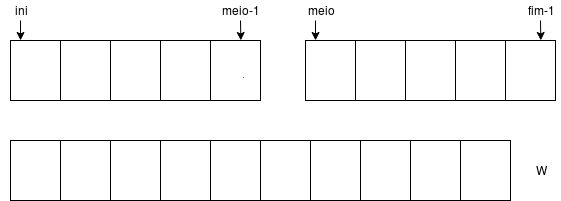
\includegraphics[width=200pt]{imgs/merge/merge_vetores.png}
  \label{fig_merge_vetores}
\end{figure}
\end{frame}

%------------------------------------------------

\begin{frame}{Mergesort}{Intercalação}
Utilizaremos três variáveis para percorrer os vetores:
\begin{itemize}
\item $i$ percorre o vetor da esquerda, indicando o próximo elemento a ser inserido em $W$.
\item $j$ percorre o vetor da direita, indicando o próximo elemento a ser inserido em $W$.
\item $k$ indica a posição em que o elemento deve ser inserido em $W$.
\end{itemize}
\begin{figure}[!h]
  \centering
  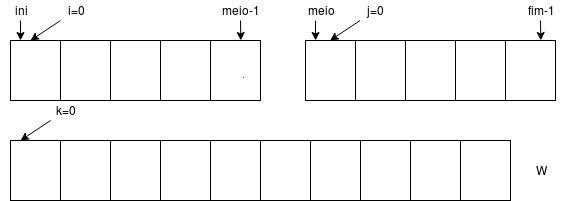
\includegraphics[width=250pt]{imgs/merge/merge0.png}
  \label{fig_merge0}
\end{figure}
\end{frame}

%------------------------------------------------

\begin{frame}[fragile]{Mergesort}{Intercalação}
\begin{itemize}
\item A intercalação acaba quando $i = meio$ ou $j = fim$.
\item A cada passo, comparamos o elemento na posição $i$ com o elemento na posição $j$, selecionando o menor e inserindo em $W$.
\item Em seguida, incremente os respectivos índice ($i$ ou $j$ e $k$).
\end{itemize}

\begin{algorithm}[H]
	$i \leftarrow ini$; 
	$j \leftarrow meio$;
	$k \leftarrow 0$\\
	\Enqto {( $i < meio$ AND $j < fim$)} {
		\Se{$V[i] \leq V[j]$} {
			$W[k] \leftarrow V[i]$ \\
			$i \leftarrow i + 1$\\
		}
		\Senao{
			$W[k] \leftarrow V[j]$ \\
			$j \leftarrow j + 1$\\
		}
		$k \leftarrow k +1$
	}
\end{algorithm}
\end{frame}

%------------------------------------------------

\begin{frame}{Mergesort}{Intercalação}
Considere como exemplo a intercalação dos dois vetores. 
\begin{enumerate}
 \item Compara-se 3 com 1. 
\end{enumerate}

\begin{figure}[!h]
  \centering
  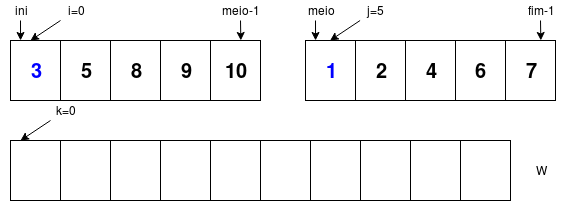
\includegraphics[width=250pt]{imgs/merge/merge1.png}
  \label{fig_merge1}
\end{figure}
\end{frame}

%------------------------------------------------

\begin{frame}{Mergesort}{Intercalação}
Considere como exemplo a intercalação dos dois vetores. 
\begin{enumerate}
 \item Compara-se 3 com 1.
 \item Insere o menor (1) em $W$.
\end{enumerate}

\begin{figure}[!h]
  \centering
  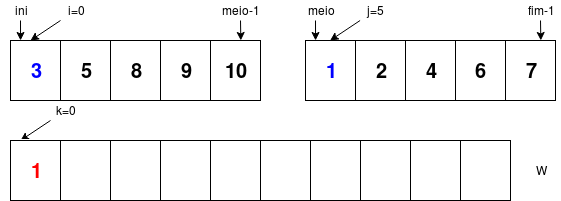
\includegraphics[width=250pt]{imgs/merge/merge1_1.png}
  \label{fig_merge1_1}
\end{figure}
\end{frame}

%------------------------------------------------

\begin{frame}{Mergesort}{Intercalação}
Considere como exemplo a intercalação dos dois vetores. 
\begin{enumerate}
 \item Compara-se 3 com 1.
 \item Insere o menor (1) em $W$.
 \item Por fim, incrementa-se $j$ e $k$ :
\end{enumerate}
 \begin{itemize}
 \item $j\leftarrow 5 +1$
 \item $k\leftarrow 0 + 1$
 \end{itemize} 

\begin{figure}[!h]
  \centering
  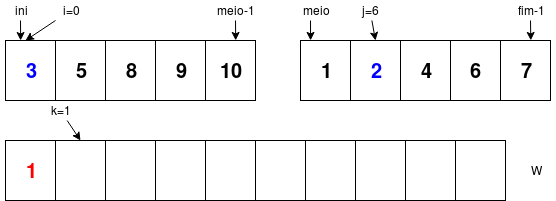
\includegraphics[width=250pt]{imgs/merge/merge2.png}
  \label{fig_merge1_2}
\end{figure}
\end{frame}
%------------------------------------------------

\begin{frame}{Mergesort}{Intercalação}
\begin{enumerate}
 \item Compara-se 3 com 2.
\end{enumerate}

\begin{figure}[!h]
  \centering
  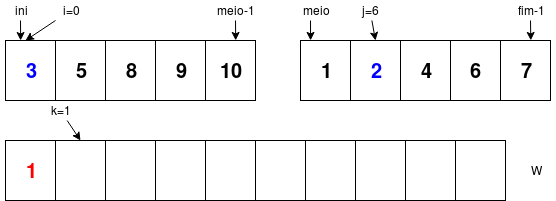
\includegraphics[width=250pt]{imgs/merge/merge2.png}
  \label{fig_merge2}
\end{figure}
\end{frame}

%------------------------------------------------

\begin{frame}{Mergesort}{Intercalação}
\begin{enumerate}
 \item Compara-se 3 com 2.
 \item Insere o menor (2) em $W$.
\end{enumerate}

\begin{figure}[!h]
  \centering
  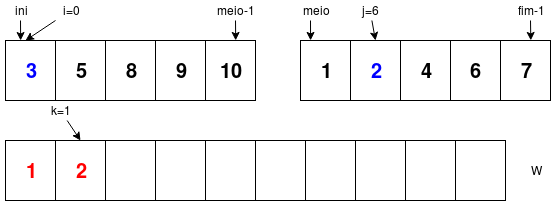
\includegraphics[width=250pt]{imgs/merge/merge2_1.png}
  \label{fig_merge2_1}
\end{figure}
\end{frame}

%------------------------------------------------

\begin{frame}{Mergesort}{Intercalação}
\begin{enumerate}
 \item Compara-se 3 com 2.
 \item Insere o menor (2) em $W$.
 \item Por fim, incrementa-se $j$ e $k$.
 \begin{itemize}
 \item $j\leftarrow 6 +1$
 \item $k\leftarrow 1 + 1$
 \end{itemize}  
\end{enumerate}

\begin{figure}[!h]
  \centering
  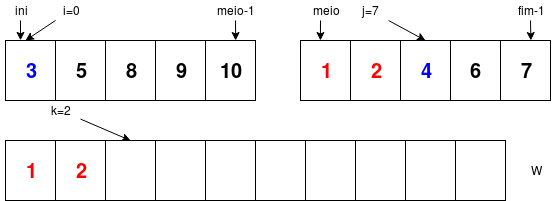
\includegraphics[width=250pt]{imgs/merge/merge3.png}
  \label{fig_merge2_2}
\end{figure}
\end{frame}

%------------------------------------------------

\begin{frame}{Mergesort}{Intercalação}
\begin{enumerate}
 \item Compara-se 3 com 4. 
\end{enumerate}

\begin{figure}[!h]
  \centering
  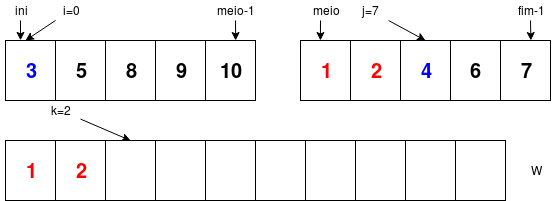
\includegraphics[width=250pt]{imgs/merge/merge3.png}
  \label{fig_merge3}
\end{figure}
\end{frame}

%------------------------------------------------

\begin{frame}{Mergesort}{Intercalação}
\begin{enumerate}
 \item Compara-se 3 com 4.
 \item Insere o menor (3) em $W$.   
\end{enumerate}

\begin{figure}[!h]
  \centering
  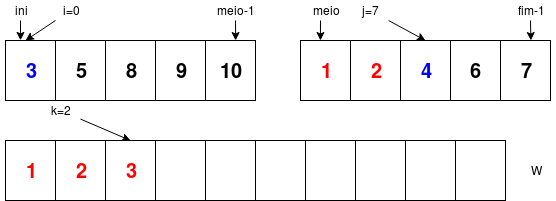
\includegraphics[width=250pt]{imgs/merge/merge3_1.png}
  \label{fig_merge3_1}
\end{figure}
\end{frame}

%------------------------------------------------

\begin{frame}{Mergesort}{Intercalação}
\begin{enumerate}
 \item Compara-se 3 com 4.
 \item Insere o menor (3) em $W$.
 \item Em seguida, incrementa-se $i$ e $k$.
 \begin{itemize}
 \item $i\leftarrow 0 + 1$
 \item $k\leftarrow 2 + 1$
 \end{itemize}   
\end{enumerate}

\begin{figure}[!h]
  \centering
  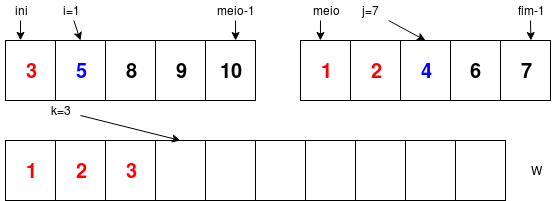
\includegraphics[width=250pt]{imgs/merge/merge4.png}
  \label{fig_merge3_2}
\end{figure}
\end{frame}


%------------------------------------------------

\begin{frame}{Mergesort}{Intercalação}
\begin{enumerate}
 \item Compara-se 5 com 4.
\end{enumerate}

\begin{figure}[!h]
  \centering
  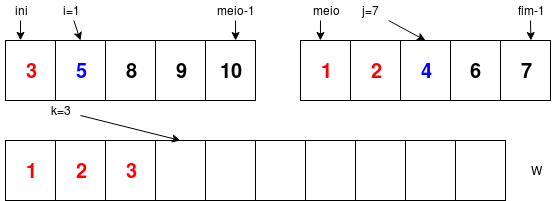
\includegraphics[width=250pt]{imgs/merge/merge4.png}
  \label{fig_merge4}
\end{figure}
\end{frame}

%------------------------------------------------

\begin{frame}{Mergesort}{Intercalação}
\begin{enumerate}
 \item Compara-se 5 com 4.
 \item Insere o menor (4) em $W$.
\end{enumerate}

\begin{figure}[!h]
  \centering
  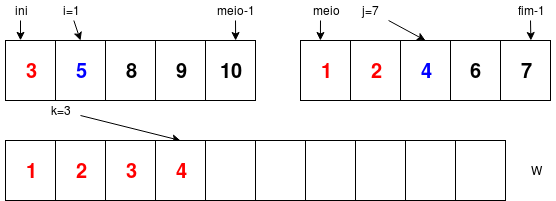
\includegraphics[width=250pt]{imgs/merge/merge4_1.png}
  \label{fig_merge4_1}
\end{figure}
\end{frame}

%------------------------------------------------

\begin{frame}{Mergesort}{Intercalação}
\begin{enumerate}
 \item Compara-se 5 com 4.
 \item Insere o menor (4) em $W$.
 \item Em seguida, incrementa-se $j$ e $k$.
 \begin{itemize}
 \item $j\leftarrow 7 + 1$
 \item $k\leftarrow 3 + 1$
 \end{itemize}  
\end{enumerate}

\begin{figure}[!h]
  \centering
  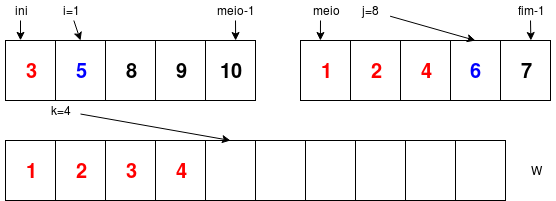
\includegraphics[width=250pt]{imgs/merge/merge5.png}
  \label{fig_merge4_2}
\end{figure}
\end{frame}
%------------------------------------------------

\begin{frame}{Mergesort}{Intercalação}
\begin{enumerate}
 \item Compara-se 5 com 6.
\end{enumerate}

\begin{figure}[!h]
  \centering
  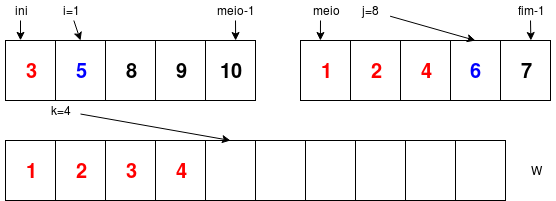
\includegraphics[width=250pt]{imgs/merge/merge5.png}
  \label{fig_merge5}
\end{figure}
\end{frame}

%------------------------------------------------

\begin{frame}{Mergesort}{Intercalação}
\begin{enumerate}
 \item Compara-se 5 com 6.
 \item Insere o menor (5) em $W$.
\end{enumerate}

\begin{figure}[!h]
  \centering
  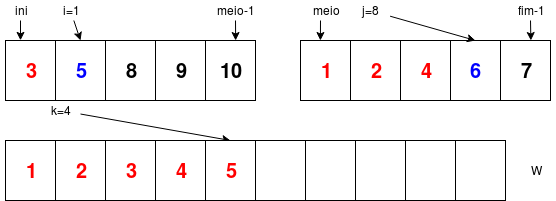
\includegraphics[width=250pt]{imgs/merge/merge5_1.png}
  \label{fig_merge5_1}
\end{figure}
\end{frame}

%------------------------------------------------

\begin{frame}{Mergesort}{Intercalação}
\begin{enumerate}
 \item Compara-se 5 com 6.
 \item Insere o menor (5) em $W$.
 \item Em seguida, incrementa-se $i$ e $k$.
 \begin{itemize}
 \item $i\leftarrow 1 + 1$
 \item $k\leftarrow 4 + 1$
 \end{itemize}   
\end{enumerate}

\begin{figure}[!h]
  \centering
  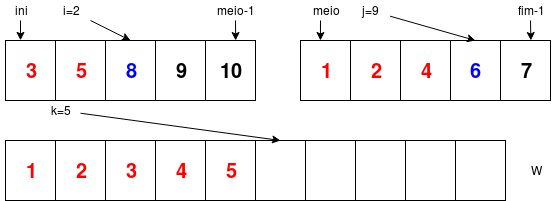
\includegraphics[width=250pt]{imgs/merge/merge6.png}
  \label{fig_merge5_2}
\end{figure}
\end{frame}

%------------------------------------------------

\begin{frame}{Mergesort}{Intercalação}
\begin{enumerate}
 \item Compara-se 8 com 6.
\end{enumerate}

\begin{figure}[!h]
  \centering
  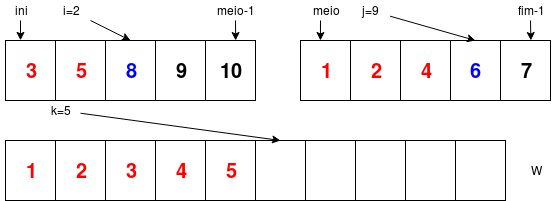
\includegraphics[width=250pt]{imgs/merge/merge6.png}
  \label{fig_merge6}
\end{figure}
\end{frame}

%------------------------------------------------

\begin{frame}{Mergesort}{Intercalação}
\begin{enumerate}
 \item Compara-se 8 com 6.
 \item Insere o menor (6) em $W$. 
\end{enumerate}

\begin{figure}[!h]
  \centering
  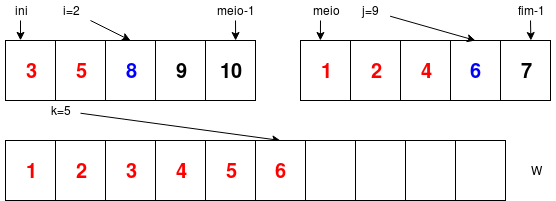
\includegraphics[width=250pt]{imgs/merge/merge6_1.png}
  \label{fig_merge6_1}
\end{figure}
\end{frame}

%------------------------------------------------

\begin{frame}{Mergesort}{Intercalação}
\begin{enumerate}
 \item Compara-se 8 com 6.
 \item Insere o menor (6) em $W$.
 \item Em seguida, incrementa-se $j$ e $k$.
 \begin{itemize}
 \item $j\leftarrow 8 + 1$
 \item $k\leftarrow 5 + 1$
 \end{itemize}  
\end{enumerate}

\begin{figure}[!h]
  \centering
  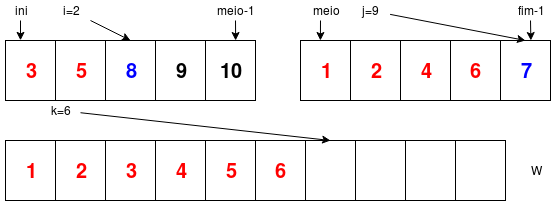
\includegraphics[width=250pt]{imgs/merge/merge7.png}
  \label{fig_merge6_2}
\end{figure}
\end{frame}

%------------------------------------------------

\begin{frame}{Mergesort}{Intercalação}
\begin{enumerate}
 \item Compara-se 8 com 7.
\end{enumerate}

\begin{figure}[!h]
  \centering
  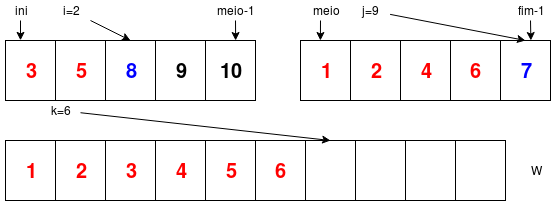
\includegraphics[width=250pt]{imgs/merge/merge7.png}
  \label{fig_merge7}
\end{figure}
\end{frame}

%------------------------------------------------

\begin{frame}{Mergesort}{Intercalação}
\begin{enumerate}
 \item Compara-se 8 com 7.
 \item Insere o menor (7) em $W$.
\end{enumerate}

\begin{figure}[!h]
  \centering
  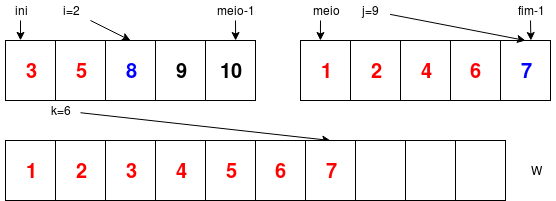
\includegraphics[width=250pt]{imgs/merge/merge7_1.png}
  \label{fig_merge7_1}
\end{figure}
\end{frame}

%------------------------------------------------

\begin{frame}{Mergesort}{Intercalação}
\begin{enumerate}
 \item Compara-se 8 com 7.
 \item Insere o menor (7) em $W$.
 \item Em seguida, incrementa-se $j$ e $k$.
 \begin{itemize}
 \item $j\leftarrow 9 + 1$
 \item $k\leftarrow 6 + 1$
 \end{itemize}  
\end{enumerate}

\begin{figure}[!h]
  \centering
  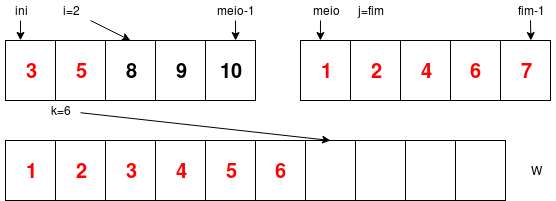
\includegraphics[width=250pt]{imgs/merge/merge8.png}
  \label{fig_merge7_2}
\end{figure}
\end{frame}


%------------------------------------------------

\begin{frame}{Mergesort}{Intercalação}
\begin{enumerate}
 \item Todos os elementos do vetor da direita foram inseridos em $W$.
 \item A condição ``{\bf Enquanto }$(i<meio$ AND $j<fim)$'' não é mais verdadeira.
 \begin{itemize}
 \item pois $j=fim$, ou seja, atingiu o fim do vetor.
 \end{itemize}
 \item Mas ainda falta inserir os elementos que restam no vetor da esquerda.
\end{enumerate}

\begin{figure}[!h]
  \centering
  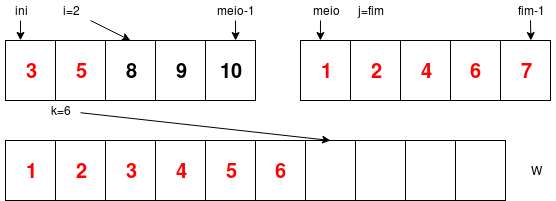
\includegraphics[width=250pt]{imgs/merge/merge8.png}
  \label{fig_merge8}
\end{figure}
\end{frame}

%------------------------------------------------

\begin{frame}{Mergesort}{Intercalação}
\begin{itemize}
\item Quando um dos dois vetores não tiver mais elementos, deve-se copiar os elementos restantes para o vetor $W$. 
\item O código a seguir realiza essa operação para ambos os vetores (da esquerda e da direita).
\end{itemize}
\begin{algorithm}[H]
	\Enqto {($i<meio$)}{
		$W[k] \leftarrow V[i]$\\
		$i \leftarrow i + 1$\\
		$k \leftarrow k + 1$\\
	}
	\Enqto {($j<fim$)}{
		$W[k] \leftarrow V[j]$\\
		$j \leftarrow j + 1$\\
		$k \leftarrow k + 1$\\
	}	
\end{algorithm}
\end{frame}

%------------------------------------------------

\begin{frame}{Mergesort}{Intercalação}
\begin{itemize}
 \item Ao copiar todos os elementos restantes para $W$, o vetor $W$ estará ordenado.

\begin{figure}[!h]
  \centering
  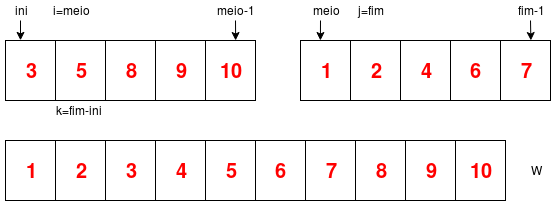
\includegraphics[width=250pt]{imgs/merge/merge9.png}
  \label{fig_merge9}
\end{figure}

\item Mas ainda resta copiar os elementos de $W$ para $V$, pois o algoritmo ordena o vetor $V$.
\end{itemize}
\end{frame}

%------------------------------------------------

\begin{frame}{Mergesort}{Intercalação}
\begin{itemize}
\item Por fim, copie os elementos de $W$ para $V$.
\begin{algorithm}[H]
	\Para {($i \leftarrow ini \textrm{ até } fim -1 $)} {
		$V[i] \leftarrow W[i- ini]$\\
	}
\end{algorithm}
\item O algoritmo completo fica conforme o pseudo-código a seguir:
\end{itemize}
\end{frame}

%------------------------------------------------

\begin{frame}{Merge}{Pseudo-código}
\scalebox{0.62}{
\begin{algorithm}[H]
\caption{Merge} 
\label{Merge}
\Entrada{Vetor $V[ini..fim-1]$, $ini$, $meio$, $fim$. }
\Saida{Vetor $V$ ordenado}
\Inicio{
      \CommentSty{// Considere o vetor auxiliar W[ini..fim-1]}\\
	$i \leftarrow ini$; 
	$j \leftarrow meio$;
	$k \leftarrow 0$\\
	\Enqto {( $i < meio$ e $j < fim$)} {
		\Se{$V[i] \leq V[j]$} {
			$W[k] \leftarrow V[i]$ \\
			$i \leftarrow i + 1$\\
		}
		\Senao{
			$W[k] \leftarrow V[j]$ \\
			$j \leftarrow j + 1$;\\
		}
		$k \leftarrow k + 1$\\
	}
	\Enqto {($i<meio$)}{
		$W[k] \leftarrow V[i]$\\
		$i \leftarrow i + 1$; $k \leftarrow k + 1$\\
	}
	\Enqto {($j<fim$)}{
		$W[k] \leftarrow V[j]$\\
		$j \leftarrow j + 1$; $k \leftarrow k + 1$\\
	}	
	\Para {($i \leftarrow ini \textrm{ até } fim - 1 $)} {
		$V[i] \leftarrow W[i- ini]$\\
	}
}
\end{algorithm}
} % scalebox

\Tiny{Adaptado de \citeonline{Ziviani2011}.}
\end{frame}

%------------------------------------------------

\begin{frame}{Mergesort}{Análise}
\begin{itemize}
\item Quando um algoritmo contém chamadas recursivas, o cálculo de seu tempo de execução pode usar recorrências.
\item Para o método de Divisão e Conquista.
\item Seja $T(n)$ o tempo do algoritmo. Suponha que dividimos em a subproblemas de tamanho $\frac{n}{b}$ cada e seja $D(n)$ o tempo para dividir os subproblemas e $C(n)$ o tempo para combiná-los. Então
\end{itemize}
\begin{equation*}
    T(n) = \begin{cases}
               \Theta(1)                      & \textrm{se } n \leq c\\
               aT(\frac{n}{b}) + D(n) +C(n)  & \textrm{se } n > c \\
           \end{cases}
\end{equation*}
\end{frame}

%------------------------------------------------

\begin{frame}{Mergesort}{Análise}
\begin{itemize}
\item Dividir: Tempo Constante $\Theta(1)$.
\item Conquistar: Dois problemas de $\frac{n}{2}$ cada: $2T(\frac{n}{2})$.
\item Combinar: Tempo do Merge: $\Theta(n)$.
\begin{equation*}
    T(n) = \begin{cases}
               \Theta(1)                      & \textrm{se } n = 1\\
               2T(\frac{n}{2}) +\Theta(n)  & \textrm{se } n > 1 \\
           \end{cases}
\end{equation*}
\item Como resolver? Árvore de Recursão!
\end{itemize}
\end{frame}

%------------------------------------------------

\begin{frame}
\begin{figure}[!h]
  \centering
  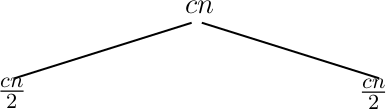
\includegraphics[width=200pt]{imgs/arvore_mergesort.png}
  \label{fig_arvore_mergesort}
\end{figure}
\end{frame}

%------------------------------------------------

\begin{frame}
\begin{figure}[!h]
  \centering
  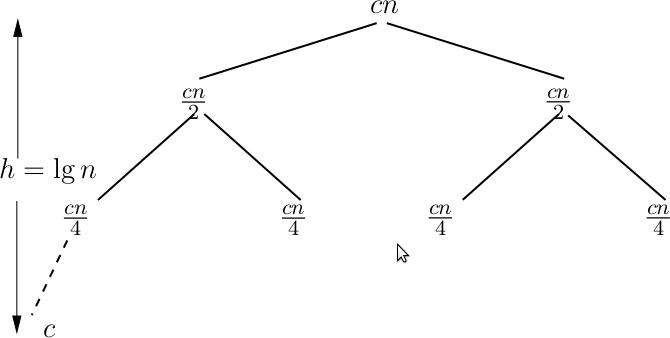
\includegraphics[width=300pt]{imgs/arvore_mergesort1.png}
  \label{fig_arvore_mergesort1}
\end{figure}
\end{frame}

%------------------------------------------------

\begin{frame}
\begin{figure}[!h]
  \centering
  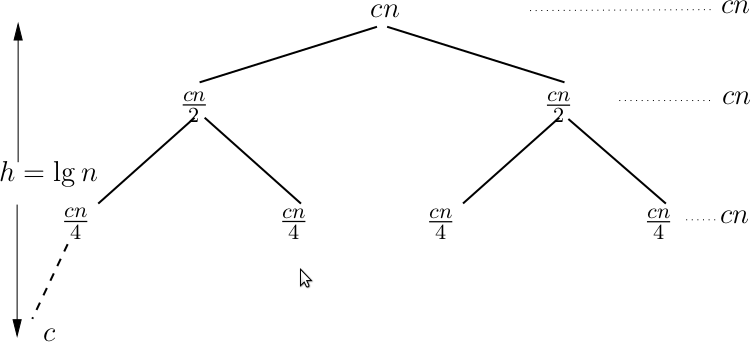
\includegraphics[width=300pt]{imgs/arvore_mergesort2.png}
  \label{fig_arvore_mergesort2}
\end{figure}
\end{frame}

%------------------------------------------------

\begin{frame}
\begin{figure}[!h]
  \centering
  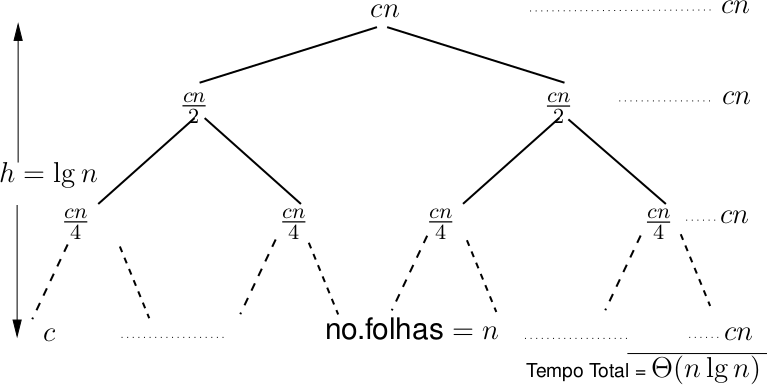
\includegraphics[width=300pt]{imgs/arvore_mergesort3.png}
  \label{fig_arvore_mergesort3}
\end{figure}
\end{frame}


%------------------------------------------------
\section{Heapsort}
%------------------------------------------------

\begin{frame}
\Huge{\centerline{Heapsort}}
\end{frame}

%------------------------------------------------

\begin{frame}{Heapsort}{Características}
\begin{itemize}
\item Possui o mesmo princípio de funcionamento da ordenação por seleção (Selectionsort).
\begin{itemize}
\item Selecione o menor item do vetor.
\item Troque-o pelo item da primeira posição.
\item Repita operação com os elementos restantes do vetor.
\end{itemize}
\item Implementação direta.
\begin{itemize}
\item Encontrar o menor elemento requer $n-1$ comparações.
\end{itemize}
\item Ideia:
\begin{itemize}
\item Utilização de uma {\it fila de prioridades} implementada com um {\bf Heap}.
\end{itemize}
\end{itemize}
\end{frame}


%------------------------------------------------

\begin{frame}{Heapsort}{Fila de Prioridades}
\begin{itemize}
\item Uma {\bf Fila de Prioridades} é um tipo abstrato de dados que permite executar as seguintes operações : 
\begin{itemize}
 \item inserir um novo item; 
 \item remover o item com a maior chave (maior prioridade).
\end{itemize}
\item A {\it chave} de cada item reflete a {\it prioridade} em que se deve tratar aquele item.
\item Aplicações:
\begin{itemize}
\item Sistemas operacionais, paginação de memória, ordenação, simulação de eventos.
\end{itemize}
\end{itemize}
\end{frame}

%------------------------------------------------

\begin{frame}{Heapsort}{Fila de Prioridades}
Operações em uma {\bf Fila de Prioridades}:
\begin{itemize}
\item Constrói uma {\it Fila de Prioridade} em um vetor de $n$ itens.
\item Insere um novo item.
\item Retira o maior item.
\item Altera a prioridade de um item.

\end{itemize}
\end{frame}

%------------------------------------------------

\begin{frame}{Heapsort}{Fila de Prioridades}
Uma {\it fila de prioridades} pode ser representada utilizando:
\begin{itemize}
\item Lista encadeada ordenada
\item Lista encadeada não ordenada
\item {\bf Heap}
\end{itemize}
\begin{figure}[!h]
  \centering
  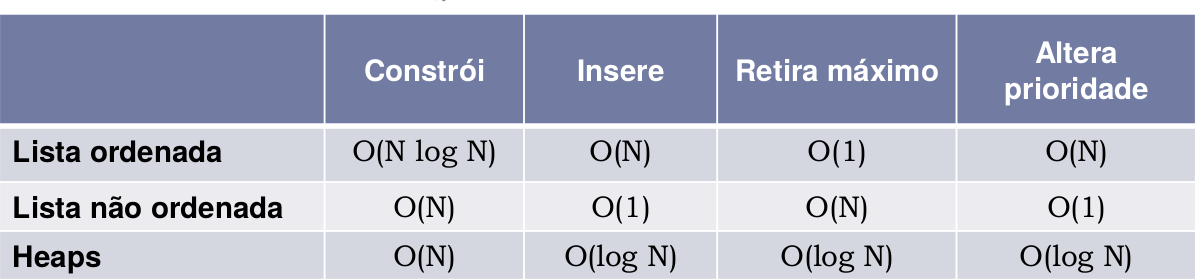
\includegraphics[width=300pt]{imgs/fila_prioridade_comparativo.png}
  \label{fig_fila_prioridade_comparativo}
\end{figure}
\end{frame}

%------------------------------------------------

\begin{frame}{Heapsort}{Fila de Prioridades}
Existem dois tipos de {\bf Heap}:
\begin{itemize}
\item {\bf Heap Máximo} - pai maior que os filhos.
\item {\bf Heap Mínimo} - pai menor que os filhos.
\item Entre os filhos não existe ordenação.
\end{itemize}
\end{frame}
%------------------------------------------------

\begin{frame}{Heapsort}{Fila de Prioridades}
Como representar um {\bf Heap}:
\begin{itemize}
\item Representação por Árvore Binária:
\begin{itemize}
\item Pai maior (ou menor) que os filhos.
\end{itemize}
\item Representação vetorial $V[0..n-1]$.
\begin{itemize}
\item {\bf Heap Máximo} - pai na posição $i$, filhos nas posições $2i+1$ e $2i+2$.
\begin{itemize}
\item $V[i] \geq V[2i+1]$ e $V[i] \geq V[2i+2]$ para todo $i$.
\end{itemize}
\item {\bf Heap Mínimo} - pai na posição $i$, filhos nas posições $2i+1$ e $2i+2$.
\begin{itemize}
\item $V[i] \leq V[2i+1]$ e $V[i] \leq V[2i+2]$ para todo $i$.
\end{itemize}
\end{itemize}
\end{itemize}

\begin{figure}[!h]
  \centering
  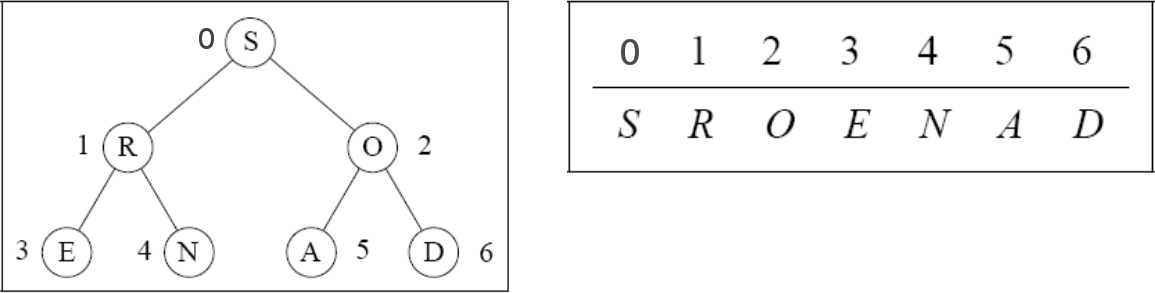
\includegraphics[width=300pt]{imgs/representacao_fila_prioridade.png}
  \label{fig_representacao_fila_prioridade}
\end{figure}
\end{frame}

%------------------------------------------------

\begin{frame}{Heapsort}{Fila de Prioridades}
Representações:
\begin{itemize}
\item Correspondência entre representação em árvore e representação em vetor.
\item Nós são numerados de 0 a $n$ .
\item O primeiro é chamado raiz.
\item O nó $\frac{k}{2}$ é o pai do nó $k$, $1 < k < n$.
\item Os nós $(2k+1)$ e $(2k+2)$ são filhos da esquerda e direita do nó $k$, para $0 \leq k < \frac{n}{2}$.
\end{itemize}

\begin{figure}[!h]
  \centering
  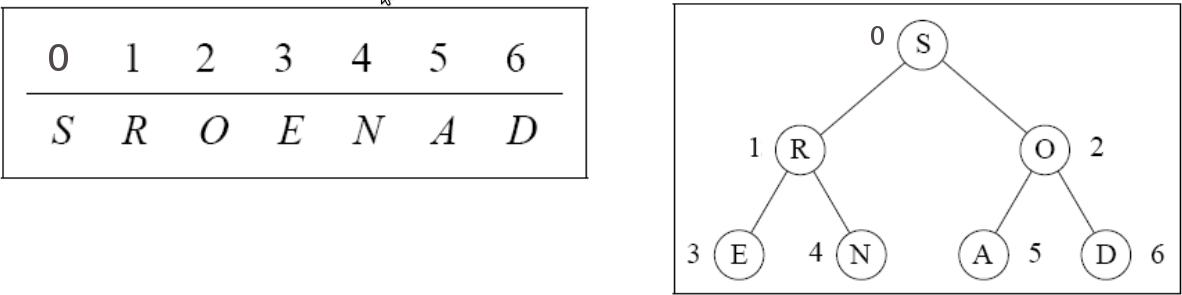
\includegraphics[width=300pt]{imgs/representacao_fila_prioridade1.png}
  \label{fig_representacao_fila_prioridade1}
\end{figure}
\end{frame}

%------------------------------------------------

\begin{frame}{Heapsort}{Fila de Prioridades}
\begin{itemize}
\item Representação por meio de vetores é compacta.
\item Permite caminhar pelos nós da árvore facilmente.
\item Filhos de um nó $i$ estão nas posições $2i+1$ e $2i + 2$.
\item O pai de um nó $i$ está na posição $\frac{i-1}{2}$.
\item A maior chave sempre está na posição 1.
\end{itemize}
\end{frame}

%------------------------------------------------

\begin{frame}{Heapsort}{Manutenção}
\begin{itemize}
\item Precisamos garantir que o valor da chave do pai é maior que dos filhos.
\item Se tiver filho maior do que o pai, troca o maior filho com o pai.
\end{itemize}
\begin{figure}[!h]
  \centering
  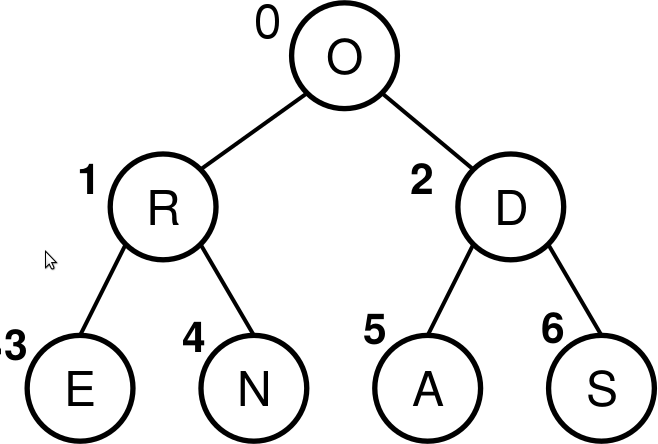
\includegraphics[width=200pt]{imgs/manutencao_fila_prioridade.png}
  \label{fig_manutencao_fila_prioridade}
\end{figure}
\end{frame}

%------------------------------------------------

\begin{frame}{Heapsort}{Manutenção}
\begin{itemize}
\item Precisamos garantir que o valor da chave do pai é maior que dos filhos.
\item Se tiver filho maior do que o pai, troca o maior filho com o pai.
\end{itemize}
\begin{figure}[!h]
  \centering
  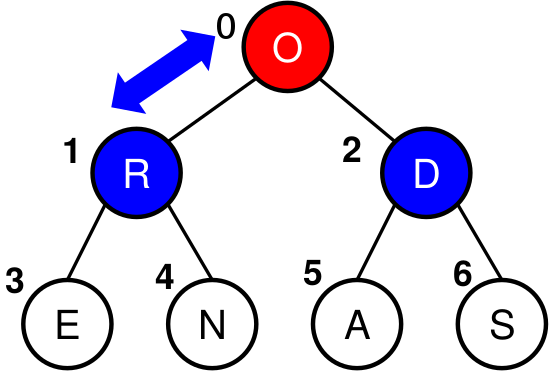
\includegraphics[width=200pt]{imgs/manutencao_fila_prioridade1.png}
  \label{fig_manutencao_fila_prioridade1}
\end{figure}
\end{frame}

%------------------------------------------------

\begin{frame}{Heapsort}{Manutenção}
\begin{itemize}
\item Precisamos garantir que o valor da chave do pai é maior que dos filhos.
\item Se tiver filho maior do que o pai, troca o maior filho com o pai.
\end{itemize}
\begin{figure}[!h]
  \centering
  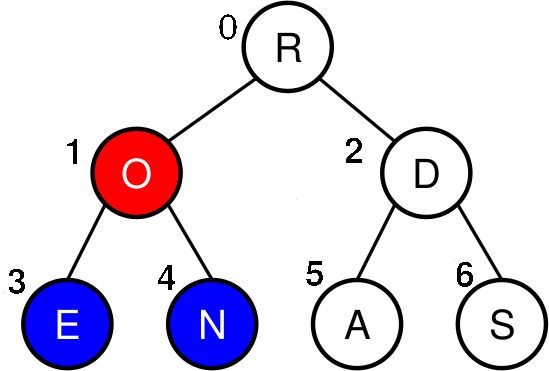
\includegraphics[width=200pt]{imgs/manutencao_fila_prioridade2.png}
  \label{fig_manutencao_fila_prioridade2}
\end{figure}
\end{frame}

%------------------------------------------------

\begin{frame}{Heapsort}{Manutenção}
\begin{itemize}
\item Precisamos garantir que o valor da chave do pai é maior que dos filhos.
\item Testa se os elementos $V[2i+1]$ e $V[2i+2]$ são menores ou igual a $V[i]$.
\item Troca com o maior filho caso contrário
\end{itemize}
\begin{figure}[!h]
  \centering
  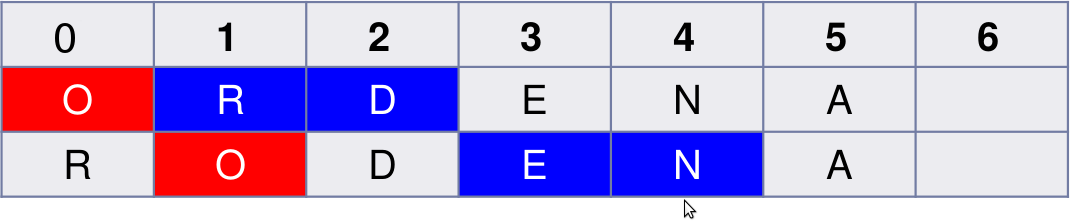
\includegraphics[width=200pt]{imgs/manutencao_fila_prioridade3.png}
  \label{fig_manutencao_fila_prioridade3}
\end{figure}
\end{frame}

%------------------------------------------------

\begin{frame}{ConstroiHeap}{Pseudo-código}
\scalebox{0.8}{
\begin{algorithm}[H]
\caption{ConstroiHeap} 
\label{ConstroiHeap}
\Entrada{Vetor $V[i..n-1]$, raiz no nó $i$, tamanho do vetor $n$}
\Saida{Heap no vetor $V[i..n-1]$}
\Inicio{
    $maior \leftarrow i$  \CommentSty{// Inicializa maior como a raiz} \\
    $l \leftarrow 2i + 1$ \CommentSty{// Filho da esquerda} \\
    $r \leftarrow 2i + 2$ \CommentSty{// Filho da direita} \\
    \CommentSty{// Se o filho da esquerda é maior que a raiz}\\
    \Se{ ( $l < n$ AND $V[l] > V[maior]$ )} {
        $maior \leftarrow l$\\
    }
    \CommentSty{// Se filho da direita é maior que a raiz}\\
    \Se{ ($r < n$ AND $V[r] > V[maior])$ }{
        $maior \leftarrow r$\\
    }
    \CommentSty{ // Se maior não é a raiz}\\
    \Se { ($maior \neq i$)}
    {
        Troca $V[i] \leftrightarrow V[maior]$ \CommentSty{ // O maior passa a ser a raiz}\\
        ConstroiHeap(V, maior, n) \CommentSty{// Cria o heap na sub-árvore}\\
    }
}
\end{algorithm}
}
\end{frame}

%------------------------------------------------

\begin{frame}{Heapsort}{Pseudo-código}
\scalebox{0.95}{
\begin{algorithm}[H]
\caption{Heapsort} 
\label{Heap}
\Entrada{Vetor $V[0..n-1]$, tamanho do vetor $n$}
\Saida{Vetor $V$ ordenado}
\Inicio{
    \CommentSty{// Contrói o heap rearranjando o vetor}\\
    \Para { ( $i \leftarrow \frac{n}{2}-1$ decrescendo até $i = 0$ )} {
        ConstroiHeap(V, i, n) \\
    }
    \CommentSty{// Extrai cada elemento, um por um, do heap}\\
    \Para {( $i\leftarrow n-1$ decrescendo até $i=0$) }
    {
        \CommentSty{// Move a raiz atual para o fim do vetor.}\\
        Troca $V[0] \leftrightarrow V[i]$\\
        \CommentSty{// Chama a função para recriar o heap} \\
        \CommentSty{// no vetor reduzido}\\
        ConstroiHeap(V, 0, i)\\
    }
}
\end{algorithm}
}
\end{frame}

%------------------------------------------------

\begin{frame}{Heapsort}{Análise}
\begin{itemize}
\item A função ConstroiHeap é chamado recursivamente no máximo $\log n$ vezes.
\item Na função Heapsort, a função ConstroiHeap é chamada dentro dos laços de repetição das linhas 3 e 6.
\begin{itemize}
\item O laço da linha 3 é executado $\frac{n}{2}$ vezes.
\item O laço da linha 6 é executado $n$ vezes.
\end{itemize}
\item Logo, o Heapsort gasta um tempo proporcional a $O(n \log n)$, no pior caso.
\end{itemize}
\end{frame}


%------------------------------------------------

\begin{frame}{Heapsort}{Vantagens x Desvantagens}
\begin{itemize}
\item Vantagens
\begin{itemize}
\item Comportamento $O(n \log n)$.
\end{itemize}
\item Desvantagens
\begin{itemize}
\item Não é estável.
\item Não é tão rápido quanto o Quicksort.
\begin{itemize}
\item A função {\bf ConstroiHeap} realiza mais operações que a função {\bf Particiona} do Quicksort.
\end{itemize}
\end{itemize}
\end{itemize}
\end{frame}

%------------------------------------------------
\section{Quicksort}
%------------------------------------------------

\begin{frame}
\Huge{\centerline{Quicksort}}
\end{frame}

\begin{frame}{Quicksort}{Características}
\begin{itemize}
\item Proposto por Hoare em 1960 e publicado em 1962.
\item É o algoritmo de ordenação interna mais rápido que se conhece para uma ampla variedade de situações.
\item Provavelmente é o mais utilizado.
\item A ideia básica é dividir o problema de ordenar um conjunto com $n$ itens em dois problemas menores.
\item Os problemas menores são ordenados independentemente.
\item Os resultados são combinados para produzir a solução final.
\end{itemize}
\end{frame}

%------------------------------------------------

\begin{frame}{Quicksort}{Características}
Método de Divisão e Conquista
\begin{itemize}
\item  A parte mais delicada do método é o processo de partição.
\item O vetor $V[Esq..Dir]$ é rearranjado por meio da escolha arbitrária de um pivô $x$.
\item O vetor V é particionado em duas partes:
\begin{itemize}
\item Parte esquerda: chaves $\leq x$.
\item Parte direita: chaves $\geq x$.
\end{itemize}
\end{itemize}
\end{frame}


%------------------------------------------------

\begin{frame}{Quicksort}{Ideia Geral}
\begin{itemize}
\item Algoritmo para o particionamento:
\begin{enumerate}
\item Escolha arbitrariamente um pivô $x$.
\item Percorra o vetor a partir da {\bf esquerda} para a {\bf direita} até que $V[i] \geq x$.
\item Percorra o vetor a partir da {\bf direita} para a {\bf esquerda} até que $V[j] \leq x$.
\item Troque $V[i]$ com $V[j]$.
\item Continue este processo até os apontadores $i$ e $j$ se cruzarem.
\end{enumerate}
\end{itemize}
\end{frame}

%------------------------------------------------

\begin{frame}{Quicksort}{Ideia Geral}
\begin{itemize}
\item Ao final do algoritmo de partição, o vetor $V[Esq..Dir]$ está particionado de tal forma que:
\begin{itemize}
\item Os itens em $V[Esq], V[Esq + 1], ... , V[j]$ são menores ou iguais a $x$.
\item Os itens em $V[i], V[i + 1], ..., V[Dir]$ são maiores ou iguais a $x$.
\end{itemize}
\end{itemize}
\end{frame}


%------------------------------------------------

\begin{frame}{Quicksort}{Exemplo}
\begin{itemize}
\item Como exemplo, considere o vetor $V[0..10]$, de tamanho $n=11$, a seguir.

\begin{figure}[!h]
  \centering
  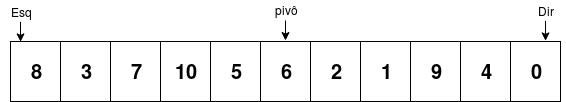
\includegraphics[width=250pt]{imgs/quick/quick1.png}
  \label{fig_quick1}
\end{figure}

 \item As variáveis {\bf Esq} e {\bf Dir} delimitam o vetor.
 \item Vamos utilizar o {\bf Pivô} como o elemento do meio.
\end{itemize}
\end{frame}

%------------------------------------------------

\begin{frame}{Quicksort}{Exemplo}
\begin{itemize}
\item Inicializa-se as variáveis auxiliares $i$ e $j$.
\begin{itemize}
 \item $i \leftarrow Esq$. 
 \begin{itemize}
 \item Irá percorrer o vetor da {\bf Esq} para a {\bf Dir}.
 \item Ou seja, será incrementado: $i\leftarrow i + 1$.
 \end{itemize}
 \item $j \leftarrow Dir$. 
 \begin{itemize}
 \item Irá percorrer o vetor da {\bf Dir} para a {\bf Esq}.
 \item Ou seja, será decrementado: $j\leftarrow j - 1$.
 \end{itemize}
\end{itemize}
\item Calcula-se o {\bf Pivô} $x\leftarrow V[ \frac{(Esq + Dir)}{2}]$
\end{itemize}

\begin{figure}[!h]
  \centering
  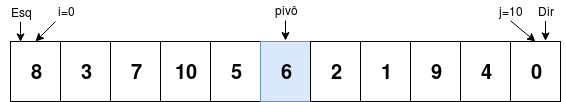
\includegraphics[width=250pt]{imgs/quick/quick2.png}
  \label{fig_quick2}
\end{figure}
\end{frame}

%------------------------------------------------

\begin{frame}{Quicksort}{Exemplo}
\begin{itemize}
 \item Verifica se o elemento na posição $i$ é \underline{maior} que o {\bf Pivô}.
 \begin{itemize}
 \item Se {\bf verdadeiro}, pára.
 \end{itemize}
 \item Verifica se o elemento na posição $j$ é \underline{menor} que o {\bf Pivô}.
 \begin{itemize}
 \item Se {\bf verdadeiro}, pára.
 \end{itemize}
\end{itemize}

\begin{figure}[!h]
  \centering
  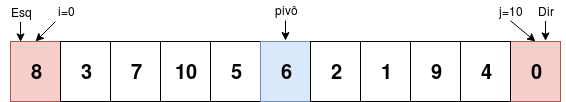
\includegraphics[width=250pt]{imgs/quick/quick3.png}
  \label{fig_quick3}
\end{figure}
\end{frame}

%------------------------------------------------

\begin{frame}{Quicksort}{Exemplo}
\begin{itemize}
 \item Troca o elemento na posição $i$ com o elemento na posição $j$.
 \begin{itemize}
 \item $V[0] \leftrightarrow V[10]$.
 \end{itemize}
 \item Em seguida, incrementa $i$ e decrementa $j$.
 \begin{itemize}
 \item $i \leftarrow 0 + 1$
 \item $j \leftarrow 10 - 1$ 
 \end{itemize} 
\end{itemize}

\begin{figure}[!h]
  \centering
  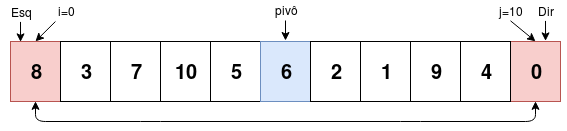
\includegraphics[width=250pt]{imgs/quick/quick4.png}
  \label{fig_quick4}
\end{figure}
\end{frame}

%------------------------------------------------

\begin{frame}{Quicksort}{Exemplo}
\begin{itemize}
 \item Verifica se o elemento na posição $i$ é \underline{maior} que o {\bf Pivô}.
 \begin{itemize}
 \item Se {\bf falso}, incrementa $i \leftarrow 1 + 1$.
 \end{itemize}
 \item Verifica se o elemento na posição $j$ é \underline{menor} que o {\bf Pivô}.
 \begin{itemize}
 \item Se {\bf verdadeiro}, pára.
 \end{itemize}
\end{itemize}

\begin{figure}[!h]
  \centering
  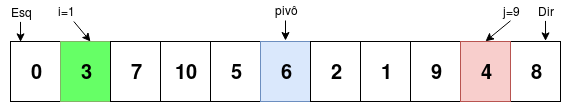
\includegraphics[width=250pt]{imgs/quick/quick5.png}
  \label{fig_quick5}
\end{figure}
\end{frame}

%------------------------------------------------

\begin{frame}{Quicksort}{Exemplo}
\begin{itemize}
 \item Verifica se o elemento na posição $i$ é \underline{maior} que o {\bf Pivô}.
 \item Verifica se o elemento na posição $j$ é \underline{menor} que o {\bf Pivô}.
 \item Se {\bf verdadeiro}, pára.
\end{itemize}

\begin{figure}[!h]
  \centering
  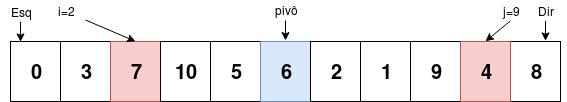
\includegraphics[width=250pt]{imgs/quick/quick6.png}
  \label{fig_quick6}
\end{figure}
\end{frame}

%------------------------------------------------

\begin{frame}{Quicksort}{Exemplo}
\begin{itemize}
 \item Troca o elemento na posição $i$ com o elemento na posição $j$.
 \begin{itemize}
 \item $V[2] \leftrightarrow V[9]$.
 \end{itemize}
 \item Em seguida, incrementa $i$ e decrementa $j$.
 \begin{itemize}
 \item $i \leftarrow 2 + 1$
 \item $j \leftarrow 9 - 1$ 
 \end{itemize} 
\end{itemize}

\begin{figure}[!h]
  \centering
  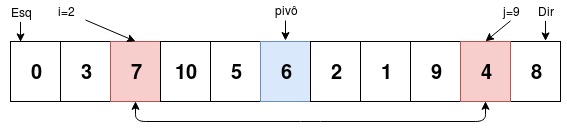
\includegraphics[width=250pt]{imgs/quick/quick7.png}
  \label{fig_quick7}
\end{figure}
\end{frame}


%------------------------------------------------

\begin{frame}{Quicksort}{Exemplo}
\begin{itemize}
 \item Verifica se o elemento na posição $i$ é \underline{maior} que o {\bf Pivô}.
 \begin{itemize}
  \item Se {\bf verdadeiro}, pára.
 \end{itemize}
 \item Verifica se o elemento na posição $j$ é \underline{menor} que o {\bf Pivô}.
 \begin{itemize}
 \item Se {\bf falso}, decrementa $j \leftarrow 8 - 1$.
 \end{itemize}
\end{itemize}

\begin{figure}[!h]
  \centering
  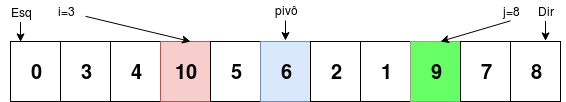
\includegraphics[width=250pt]{imgs/quick/quick8.png}
  \label{fig_quick8}
\end{figure}
\end{frame}

%------------------------------------------------

\begin{frame}{Quicksort}{Exemplo}
\begin{itemize}
 \item Verifica se o elemento na posição $i$ é \underline{maior} que o {\bf Pivô}.
 \item Verifica se o elemento na posição $j$ é \underline{menor} que o {\bf Pivô}.
 \item Se {\bf verdadeiro}, pára.
\end{itemize}
\begin{figure}[!h]
  \centering
  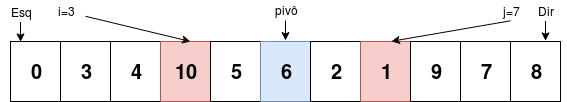
\includegraphics[width=250pt]{imgs/quick/quick9.png}
  \label{fig_quick9}
\end{figure}
\end{frame}

%------------------------------------------------

\begin{frame}{Quicksort}{Exemplo}
\begin{itemize}
 \item Troca o elemento na posição $i$ com o elemento na posição $j$.
 \begin{itemize}
 \item $V[3] \leftrightarrow V[7]$.
 \end{itemize}
 \item Em seguida, incrementa $i$ e decrementa $j$.
 \begin{itemize}
 \item $i \leftarrow 3 + 1$
 \item $j \leftarrow 7 - 1$ 
 \end{itemize} 
\end{itemize}

\begin{figure}[!h]
  \centering
  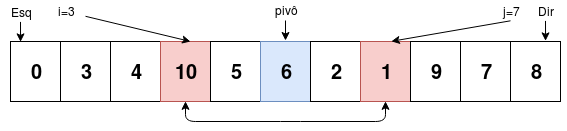
\includegraphics[width=250pt]{imgs/quick/quick10.png}
  \label{fig_quick10}
\end{figure}
\end{frame}

%------------------------------------------------

\begin{frame}{Quicksort}{Exemplo}
\begin{itemize}
 \item Verifica se o elemento na posição $i$ é \underline{maior} que o {\bf Pivô}.
 \begin{itemize}
 \item Se {\bf falso}, incrementa $i \leftarrow 4 + 1$.
 \end{itemize}
 \item Verifica se o elemento na posição $j$ é \underline{menor} que o {\bf Pivô}.
 \begin{itemize}
 \item Se {\bf verdadeiro}, pára.
 \end{itemize}
\end{itemize}

\begin{figure}[!h]
  \centering
  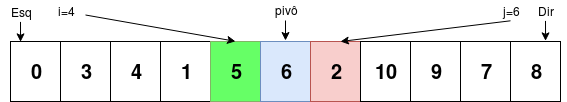
\includegraphics[width=250pt]{imgs/quick/quick11.png}
  \label{fig_quick11}
\end{figure}
\end{frame}

%------------------------------------------------

\begin{frame}{Quicksort}{Exemplo}
\begin{itemize}
 \item Verifica se o elemento na posição $i$ é \underline{maior} que o {\bf Pivô}.
 \item Verifica se o elemento na posição $j$ é \underline{menor} que o {\bf Pivô}.
 \begin{itemize}
 \item Se {\bf verdadeiro}, pára.
 \end{itemize}
\end{itemize}

\begin{figure}[!h]
  \centering
  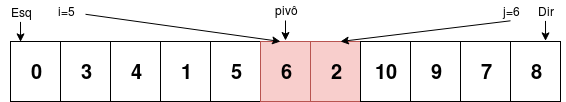
\includegraphics[width=250pt]{imgs/quick/quick12.png}
  \label{fig_quick12}
\end{figure}
\end{frame}

%------------------------------------------------

\begin{frame}{Quicksort}{Exemplo}
\begin{itemize}
 \item Troca o elemento na posição $i$ com o elemento na posição $j$.
 \begin{itemize}
 \item $V[5] \leftrightarrow V[6]$.
 \end{itemize}
 \item Em seguida, incrementa $i$ e decrementa $j$.
 \begin{itemize}
 \item $i \leftarrow 5 + 1$
 \item $j \leftarrow 6 - 1$ 
 \end{itemize} 
\end{itemize}

\begin{figure}[!h]
  \centering
  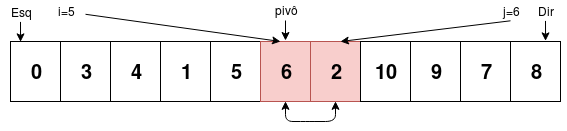
\includegraphics[width=250pt]{imgs/quick/quick13.png}
  \label{fig_quick13}
\end{figure}
\end{frame}

%------------------------------------------------

\begin{frame}{Quicksort}{Exemplo}
\begin{itemize}
 \item O processo é interrompido quando $i$ e $j$ se cruzam.
 \begin{itemize}
 \item Ou seja, $i > j$.
 \end{itemize} 


\begin{figure}[!h]
  \centering
  \includegraphics[width=250pt]{imgs/quick/quick14.png}
  \label{fig_quick14}
\end{figure}

\item Em seguida, os vetores são divididos em dois e ordena-se recursivamente cada vetor.
\begin{itemize}
\item O vetor da esquerda $V[Esq .. j]$, começa em $Esq$ e termina em $j$.
\item O vetor da direita $V[i .. Dir]$, começa em $i$ e termina em $Dir$.
\end{itemize}
\end{itemize}
\end{frame}

%------------------------------------------------

\begin{frame}{Quicksort}{Exemplo}
\begin{itemize}
 \item Realiza-se uma chamada recursiva para o vetor da esquerda $V[Esq .. j]$
 \begin{itemize}
 \item Quicksort(V,0,5)
 \end{itemize}
 \item e uma chamada recursiva para o vetor da direita $V[i .. Dir]$
 \begin{itemize}
 \item Quicksort(V,6,10)
 \end{itemize} 
\end{itemize}

\begin{figure}[!h]
  \centering
  \includegraphics[width=250pt]{imgs/quick/quick15.png}
  \label{fig_quick15}
\end{figure}
\end{frame}

%------------------------------------------------

\begin{frame}{Quicksort}{Exemplo}
Ordenando recursivamente o vetor da esquerda:
\begin{itemize}
\item Inicializa-se as variáveis auxiliares $i$ e $j$.
\begin{itemize}
 \item $i \leftarrow Esq$. 
 \item $j \leftarrow Dir$. 
\end{itemize}
\item Calcula-se o {\bf Pivô} $x\leftarrow V[ \frac{(Esq + Dir)}{2}]$
\item Verifica se o elemento na posição $i$ é \underline{maior} que o {\bf Pivô}.
\begin{itemize}
\item Se {\bf falso}, incrementa $i \leftarrow 0 + 1$.
\end{itemize} 
\item Verifica se o elemento na posição $j$ é \underline{menor} que o {\bf Pivô}.
\begin{itemize}
\item Se {\bf verdadeiro}, pára.
\end{itemize} 
\end{itemize}

\begin{figure}[!h]
  \centering
  \includegraphics[width=130pt]{imgs/quick/quick16.png}
  \label{fig_quick16}
\end{figure}
\end{frame}

%------------------------------------------------

\begin{frame}{Quicksort}{Exemplo}
\begin{itemize}
 \item Verifica se o elemento na posição $i$ é \underline{maior} que o {\bf Pivô}.
 \begin{itemize}
 \item Se {\bf falso}, , incrementa $i \leftarrow 1 + 1$.
 \end{itemize} 
 \item Verifica se o elemento na posição $j$ é \underline{menor} que o {\bf Pivô}.
 \begin{itemize}
 \item Se {\bf verdadeiro}, pára.
 \end{itemize}
\end{itemize}

\begin{figure}[!h]
  \centering
  \includegraphics[width=130pt]{imgs/quick/quick17.png}
  \label{fig_quick17}
\end{figure}
\end{frame}

%------------------------------------------------

\begin{frame}{Quicksort}{Exemplo}
\begin{itemize}
 \item Verifica se o elemento na posição $i$ é \underline{maior} que o {\bf Pivô}. 
 \item Verifica se o elemento na posição $j$ é \underline{menor} que o {\bf Pivô}.
 \item Se {\bf verdadeiro}, pára.
\end{itemize}

\begin{figure}[!h]
  \centering
  \includegraphics[width=130pt]{imgs/quick/quick18.png}
  \label{fig_quick18}
\end{figure}
\end{frame}
%------------------------------------------------

\begin{frame}{Quicksort}{Exemplo}
\begin{itemize}
 \item Troca o elemento na posição $i$ com o elemento na posição $j$.
 \begin{itemize}
 \item $V[2] \leftrightarrow V[5]$.
 \end{itemize}
 \item Em seguida, incrementa $i$ e decrementa $j$.
 \begin{itemize}
 \item $i \leftarrow 2 + 1$
 \item $j \leftarrow 5 - 1$ 
 \end{itemize} 
\end{itemize}

\begin{figure}[!h]
  \centering
  \includegraphics[width=130pt]{imgs/quick/quick19.png}
  \label{fig_quick19}
\end{figure}
\end{frame}

%------------------------------------------------

\begin{frame}{Quicksort}{Exemplo}
\begin{itemize}
 \item Verifica se o elemento na posição $i$ é \underline{maior} que o {\bf Pivô}.
  \begin{itemize}
 \item Se {\bf falso}, incrementa $i\leftarrow i + 1$.
 \end{itemize}
 \item Verifica se o elemento na posição $j$ é \underline{menor} que o {\bf Pivô}.
 \begin{itemize}
  \item Se {\bf falso}, decrementa $j\leftarrow j - 1$.
 \end{itemize}
\end{itemize}

\begin{figure}[!h]
  \centering
  \includegraphics[width=130pt]{imgs/quick/quick20.png}
  \label{fig_quick20}
\end{figure}
\end{frame}

%------------------------------------------------

\begin{frame}{Quicksort}{Exemplo}
\begin{itemize}
 \item O processo é interrompido quando $i$ e $j$ se cruzam.
 \begin{itemize}
 \item Ou seja, $i > j$.
 \end{itemize} 

\begin{figure}[!h]
  \centering
  \includegraphics[width=130pt]{imgs/quick/quick21.png}
  \label{fig_quick21}
\end{figure}

\item Em seguida, os vetores são divididos em dois e ordena-se recursivamente cada vetor.
\begin{itemize}
\item O vetor da esquerda $V[Esq .. j]$, começa em $Esq$ e termina em $j$.
\item O vetor da direita $V[i .. Dir]$, começa em $i$ e termina em $Dir$.
\end{itemize}
\end{itemize}
\end{frame}

%------------------------------------------------

\begin{frame}{Quicksort}{Exemplo}
\begin{itemize}
 \item Realiza-se uma chamada recursiva para o vetor da esquerda $V[Esq .. j]$
 \begin{itemize}
 \item Quicksort(V,0,3)
 \end{itemize}
 \item e uma chamada recursiva para o vetor da direita $V[i .. Dir]$
 \begin{itemize}
 \item Quicksort(V,4,5)
 \end{itemize} 
\end{itemize}


\begin{figure}[!h]
  \centering
  \includegraphics[width=130pt]{imgs/quick/quick22.png}
  \label{fig_quick22}
\end{figure}

\end{frame}

%------------------------------------------------

\begin{frame}{Quicksort}{Exemplo}
\begin{itemize}
 \item Inicializa-se as variáveis e calcula-se o pivô em cada vetor.
 \end{itemize}

\begin{figure}[!h]
  \centering
  \includegraphics[width=200pt]{imgs/quick/quick23.png}
  \label{fig_quick23}
\end{figure}

\end{frame}

%------------------------------------------------

\begin{frame}{Quicksort}{Exemplo}
\begin{itemize}
 \item Vetor da Esquerda:
\begin{itemize}
 \item Verifica se o elemento na posição $i$ é \underline{maior} que o {\bf Pivô}.
  \begin{itemize}
 \item Se {\bf falso}, incrementa $i\leftarrow i + 1$.
 \end{itemize}
 \item Verifica se o elemento na posição $j$ é \underline{menor} que o {\bf Pivô}.
 \begin{itemize}
  \item Se {\bf verdadeiro}, pára.
 \end{itemize}
\end{itemize}
\item Vetor da Direita:
\begin{itemize}
\item Realiza-se a mesma verificação: ambas são {\bf verdadeiras}.	
\end{itemize}
\end{itemize}
 
\begin{figure}[!h]
  \centering
  \includegraphics[width=200pt]{imgs/quick/quick24.png}
  \label{fig_quick24}
\end{figure}

\end{frame}

%------------------------------------------------

\begin{frame}{Quicksort}{Exemplo}
\begin{itemize}
 \item Vetor da Esquerda:
\begin{itemize}
 \item Verifica os elementos na posição $i$ e $j$ em relação ao pivô.
 \item Ambos os testes são {\bf verdadeiros}, o laço de repetição pára.
\end{itemize}
\item Vetor da Direita:
\begin{itemize}
\item Realiza-se a troca dos elementos.
\item Incrementa $i\leftarrow i + 1$ e decrementa $j \leftarrow j - 1$.
\end{itemize}
\end{itemize}

\begin{figure}[!h]
  \centering
  \includegraphics[width=200pt]{imgs/quick/quick25.png}
  \label{fig_quick25}
\end{figure}

\end{frame}

%------------------------------------------------

\begin{frame}{Quicksort}{Exemplo}
\begin{itemize}
 \item Vetor da Esquerda:
\begin{itemize}
 \item Realiza-se a troca dos elementos.
 \item Incrementa $i\leftarrow i + 1$ e decrementa $j \leftarrow j - 1$.
\end{itemize}
\item Vetor da Direita:
\begin{itemize}
\item $i$ e $j$ se cruzaram, laço de repetição pára.
\end{itemize}
\end{itemize}

\begin{figure}[!h]
  \centering
  \includegraphics[width=200pt]{imgs/quick/quick26.png}
  \label{fig_quick26}
\end{figure}

\end{frame}

%------------------------------------------------

\begin{frame}{Quicksort}{Exemplo}
\begin{itemize}
 \item Vetor da Esquerda:
\begin{itemize}
 \item $i$ e $j$ apontam para o mesmo elemento (Não precisa trocar).
 \item Incrementa $i\leftarrow i + 1$ e decrementa $j \leftarrow j - 1$.
\end{itemize}
\item Vetor da Direita:
\begin{itemize}
\item Ordenado.
\end{itemize}
\end{itemize}

\begin{figure}[!h]
  \centering
  \includegraphics[width=200pt]{imgs/quick/quick27.png}
  \label{fig_quick27}
\end{figure}

\end{frame}

%------------------------------------------------

\begin{frame}{Quicksort}{Exemplo}
\begin{itemize}
 \item Vetor da Esquerda:
\begin{itemize}
 \item $i$ e $j$ se cruzaram, laço de repetição pára.
 \item O vetor está ordenado.
\end{itemize}
\item Vetor da Direita:
\begin{itemize}
\item Ordenado.
\end{itemize}
\end{itemize}


\begin{figure}[!h]
  \centering
  \includegraphics[width=200pt]{imgs/quick/quick28.png}
  \label{fig_quick28}
\end{figure}

\end{frame}

%------------------------------------------------

\begin{frame}{Quicksort}{Exemplo}
Ainda falta ordenar o vetor da direita:
\begin{itemize}
 \item Inicializa as variáveis $i$ e $j$ e calcula o pivô.
\end{itemize}


\begin{figure}[!h]
  \centering
  \includegraphics[width=130pt]{imgs/quick/quick29.png}
  \label{fig_quick29}
\end{figure}

\end{frame}

%------------------------------------------------

\begin{frame}{Quicksort}{Exemplo}
\begin{itemize}
 \item Verifica se o elemento na posição $i$ é \underline{maior} que o {\bf Pivô}.
  \begin{itemize}
 \item Se {\bf falso}, incrementa $i\leftarrow i + 1$.
 \end{itemize}
 \item Verifica se o elemento na posição $j$ é \underline{menor} que o {\bf Pivô}.
 \begin{itemize}
  \item Se {\bf verdadeiro}, pára.
 \end{itemize}
\end{itemize}

\begin{figure}[!h]
  \centering
  \includegraphics[width=130pt]{imgs/quick/quick30.png}
  \label{fig_quick30}
\end{figure}

\end{frame}

%------------------------------------------------

\begin{frame}{Quicksort}{Exemplo}
\begin{itemize}
 \item Verifica se o elemento na posição $i$ é \underline{maior} que o {\bf Pivô}.
 \item Verifica se o elemento na posição $j$ é \underline{menor} que o {\bf Pivô}.
 \item Se {\bf verdadeiro}, pára.
\end{itemize}

\begin{figure}[!h]
  \centering
  \includegraphics[width=130pt]{imgs/quick/quick31.png}
  \label{fig_quick31}
\end{figure}

\end{frame}

%------------------------------------------------

\begin{frame}{Quicksort}{Exemplo}
\begin{itemize}
 \item Realiza-se a troca dos elementos.
 \item Incrementa $i\leftarrow i + 1$ e decrementa $j \leftarrow j - 1$.
\end{itemize}

\begin{figure}[!h]
  \centering
  \includegraphics[width=130pt]{imgs/quick/quick32.png}
  \label{fig_quick32}
\end{figure}

\end{frame}

%------------------------------------------------

\begin{frame}{Quicksort}{Exemplo}
\begin{itemize}
 \item Verifica se o elemento na posição $i$ é \underline{maior} que o {\bf Pivô}.
 \item Verifica se o elemento na posição $j$ é \underline{menor} que o {\bf Pivô}.
 \item Se {\bf verdadeiro}, pára.
\end{itemize}

\begin{figure}[!h]
  \centering
  \includegraphics[width=130pt]{imgs/quick/quick33.png}
  \label{fig_quick33}
\end{figure}

\end{frame}

%------------------------------------------------

\begin{frame}{Quicksort}{Exemplo}
\begin{itemize}
 \item Realiza-se a troca dos elementos.
 \item Incrementa $i\leftarrow i + 1$ e decrementa $j \leftarrow j - 1$.
\end{itemize}

\begin{figure}[!h]
  \centering
  \includegraphics[width=130pt]{imgs/quick/quick34.png}
  \label{fig_quick34}
\end{figure}

\end{frame}

%------------------------------------------------

\begin{frame}{Quicksort}{Exemplo}
\begin{itemize}
 \item $i$ e $j$ se cruzaram, laço de repetição pára.
 \item Realiza as chamadas recursivas.
\end{itemize}

\begin{figure}[!h]
  \centering
  \includegraphics[width=130pt]{imgs/quick/quick35.png}
  \label{fig_quick35}
\end{figure}

\end{frame}


%------------------------------------------------

\begin{frame}{Quicksort}{Exemplo}
\begin{itemize}
 \item Realiza uma chamada recursiva para o vetor da esquerda $V[Esq..j]$.
 \item E uma chamada recursiva para o vetor da direita $V[i..Dir]$.
\end{itemize}

\begin{figure}[!h]
  \centering
  \includegraphics[width=200pt]{imgs/quick/quick36.png}
  \label{fig_quick36}
\end{figure}

\end{frame}


%------------------------------------------------

\begin{frame}{Quicksort}{Exemplo}
\begin{itemize}
 \item Inicializa as variáveis $i$ e $j$.
 \item Calcula o pivô.
\end{itemize}

\begin{figure}[!h]
  \centering
  \includegraphics[width=200pt]{imgs/quick/quick37.png}
  \label{fig_quick37}
\end{figure}

\end{frame}


%------------------------------------------------

\begin{frame}{Quicksort}{Exemplo}
\begin{itemize}
 \item Vetor da Esquerda:
\begin{itemize}
 \item Compara os elementos nas posições $i$ e $j$ com o pivô.
 \item Incrementa $i\leftarrow i + 1$.
\end{itemize}
\item Vetor da Direita:
\begin{itemize}
\item Compara os elementos nas posições $i$ e $j$ com o pivô.
\item As condições são {\bf falsas}, incrementa $i$ e decrementa $j$.
\end{itemize}
\end{itemize}

\begin{figure}[!h]
  \centering
  \includegraphics[width=200pt]{imgs/quick/quick38.png}
  \label{fig_quick38}
\end{figure}

\end{frame}


%------------------------------------------------

\begin{frame}{Quicksort}{Exemplo}
\begin{itemize}
 \item Vetor da Esquerda:
\begin{itemize}
 \item Compara os elementos nas posições $i$ e $j$ com o pivô.
\item As condições são {\bf verdadeiras}, o laço de repetição pára.
\end{itemize}
\item Vetor da Direita:
\begin{itemize}
\item $i$ e $j$ se cruzaram, o laço de repetição pára.
\item O vetor está ordenado.
\end{itemize}
\end{itemize}

\begin{figure}[!h]
  \centering
  \includegraphics[width=200pt]{imgs/quick/quick39.png}
  \label{fig_quick39}
\end{figure}

\end{frame}


%------------------------------------------------

\begin{frame}{Quicksort}{Exemplo}
\begin{itemize}
 \item Vetor da Esquerda:
\begin{itemize}
 \item Realiza-se a troca dos elementos.
 \item Incrementa $i\leftarrow i + 1$ e decrementa $j \leftarrow j - 1$.
\end{itemize}
\item Vetor da Direita:
\begin{itemize}
\item Ordenado.
\end{itemize}
\end{itemize}

\begin{figure}[!h]
  \centering
  \includegraphics[width=200pt]{imgs/quick/quick40.png}
  \label{fig_quick40}
\end{figure}

\end{frame}


%------------------------------------------------

\begin{frame}{Quicksort}{Exemplo}
\begin{itemize}
 \item Vetor da Esquerda:
\begin{itemize}
\item $i$ e $j$ se cruzaram, o laço de repetição pára.
\item O vetor está ordenado.
\end{itemize}
\item Vetor da Direita:
\begin{itemize}
\item Ordenado.
\end{itemize}
\end{itemize}

\begin{figure}[!h]
  \centering
  \includegraphics[width=200pt]{imgs/quick/quick41.png}
  \label{fig_quick41}
\end{figure}

\end{frame}

%------------------------------------------------

\begin{frame}{QuicksortOrdena}{Pseudo-código}

\scalebox{0.9}{
\begin{algorithm}[H]
\caption{QuicksortOrdena} 
\label{QuicksortOrdena}
\Entrada{Vetor $V[0..n-1]$, tamanho $n$}
\Saida{Vetor $V$ ordenado}
\Inicio{
	Quicksort($V, 0, n-1$) \\
}
\end{algorithm}
}

\scalebox{0.9}{
\begin{algorithm}[H]
\caption{Quicksort} 
\label{Quicksort}
\Entrada{Vetor $V[Esq..Dir]$, Esq, Dir}
\Saida{Vetor $V$ ordenado}
\Inicio{
	$(i, j) \leftarrow Particiona(V, Esq, Dir)$ \\
	\Se {( $Esq < j$ ) } {
        Quicksort($V, Esq, j$ ) \\
      }
    	\Se {( $i < Dir$ )} {
        Quicksort($V, i , Dir$) \\
	}
}
\end{algorithm}
}
\end{frame}


%------------------------------------------------

\begin{frame}{Quicksort}{Pseudo-código}
\scalebox{0.8}{
\begin{algorithm}[H]
\caption{Particiona} 
\label{Particiona}
\Entrada{Vetor $V[Esq..Dir]$, Esq, Dir}
\Saida{Vetor $V$ ordenado}
\Inicio{
    $i \leftarrow Esq$; $j \leftarrow Dir$\\
    $x \leftarrow V[\frac{(i + j )}{2} ]$ \\
    \Repita{($i > j$)} { 
        \Enqto {( $x > V[ i ]$ )} { 
            $i \leftarrow i + 1$\\
        }
        \Enqto {( $x < V[ j ]$ )} { 
            $j \leftarrow j - 1$\\
        }
        \Se {( $i \leq j$ ) }
        { 
           Trocar $V[ i ] \leftrightarrow V[ j ] $\\ 
		$i \leftarrow i + 1$\\
		$j \leftarrow j - 1$\\
        }
    } 
    \Retorna $(i, j)$
}
\end{algorithm}
}

\Tiny{Adaptado de \citeonline{Ziviani2011}.}
\end{frame}


%------------------------------------------------

\begin{frame}{Quicksort}{Pseudocódigo}
\begin{itemize}
\item O laço de repetição da função Particiona é extremamente simples.
\item Razão pela qual o algoritmo Quicksort é tão rápido.
\end{itemize}
\end{frame}

%------------------------------------------------

\begin{frame}{Quicksort}{Análise}
\begin{itemize}
\item Qual o pior caso para o Quicksort?
\item Por que?
\begin{itemize}
\item Qual sua ordem de complexidade?
\item Qual o melhor caso?
\item O algoritmo é estável?
\end{itemize}
\end{itemize}
\end{frame}


%------------------------------------------------

\begin{frame}{Quicksort}{Análise}
\begin{itemize}
\item Melhor caso: $C(n) = 2C(\frac{n}{2}) + n = n \log n$
\item Ocorre quando o problema é sempre divido em subproblemas de igual tamanho após a partição.
\end{itemize}
\begin{figure}[!h]
  \centering
  \includegraphics[width=250pt]{imgs/analise_quicksort_melhorcaso.png}
  \label{fig_analise_quicksort_melhorcaso}
\end{figure} 
\end{frame}

%------------------------------------------------

\begin{frame}{Quicksort}{Análise}
\begin{itemize}
\item Pior caso: $C(n) = O(n^2)$
\item O pior caso ocorre quando, sistematicamente, o pivô é escolhido como sendo um dos extremos de um arquivo já ordenado.
\end{itemize}
\begin{figure}[!h]
  \centering
  \includegraphics[width=250pt]{imgs/analise_quicksort_piorcaso.png}
  \label{fig_analise_quicksort_piorcaso}
\end{figure} 
\end{frame}


%------------------------------------------------

\begin{frame}{Quicksort}{Análise}
\begin{itemize}
\item O pior caso pode ser evitado empregando pequenas modificações no algoritmo.
\item Para isso basta escolher três itens quaisquer do vetor e usar a mediana dos três como pivô.
\end{itemize}
\end{frame}


%------------------------------------------------

\begin{frame}{Quicksort}{Análise}
\begin{itemize}
\item Caso médio de acordo com \citeonline{Sedgewick1996}[p. 17):
\item $C(n) \approx 1,386n \log n - 0,846n$.
\item Isso significa que em média o tempo de execução do QuickSort é cerca de $O(n \log n)$.
\end{itemize}
\end{frame}


%------------------------------------------------

\begin{frame}{Quicksort}{Vantagens x Desvantagens}
\begin{itemize}
\item Vantagens:
\begin{itemize}
\item É extremamente eficiente para ordenar arquivos de dados.
\item Necessita de apenas uma pequena pilha como memória auxiliar.
\item Requer $O(n \log n)$ comparações em média (caso médio) para ordenar $n$ itens.
\end{itemize}
\item Desvantagens:
\begin{itemize}
\item Tem um pior caso $O(n^2)$ comparações.
\item Sua implementação é delicada e difícil: um pequeno engano pode levar a efeitos inesperados para algumas entradas de dados.
\item O método não é estável.
\end{itemize}
\end{itemize}
\end{frame}

%------------------------------------------------

\begin{frame}{Quicksort}{Melhorias}
\begin{itemize}
\item Pivô - mediana de três ou mediana de cinco.
\item Não empilhar quando tem apenas um item.
\item Usar algoritmo de inserção (Insertionsort) para vetores pequenos.
\item Escolha correta do lado a ser empilhado primeiro.
\item Resultado: melhoria no tempo de execução de 25\% a 30\%.
\end{itemize}
\end{frame}

%------------------------------------------------
%------------------------------------------------
\begin{frame}
\titlepage % Print the title page as the first slide

\begin{figure}[!h]
  \centering
  \includegraphics[width=80pt]{imgs/introducao.jpg}
  \label{fig_introducao}
\end{figure}
\end{frame}

%
%\begin{frame}
%\Huge{\centerline{Dúvidas}}
%
%\begin{figure}[!h]
%  \centering
%  \includegraphics[width=100pt]{imgs/dados.jpg}
%  \label{fig_fim}
%\end{figure}
%\end{frame}
%----------------------------------------------------------------------------------------
\end{document} 